\documentclass[11pt,a4paper,twoside,%
BCOR12mm,DIV14,%
headsepline,
cleardoubleempty,chapterprefix,parskip,%
liststotoc,bibtotoc]{scrbook}

% \usepackage[english, ngerman]{babel}
\usepackage[english]{babel}
\usepackage[utf8]{inputenc}
\usepackage[T1]{fontenc}
\usepackage{mathptmx}
\usepackage[scaled=0.92]{helvet}
\usepackage{courier}
\usepackage{mathtools}
\usepackage{amssymb} 
\usepackage{float}
\makeatletter
\def\displaymath{\typeout{*** Do not use DISPLAYMATH. Use \[...\] instead ***}}
\def\eqnarray{\typeout{*** Do not use EQNARRAY(*). Use align(*)-environment instead ***}}
\makeatother
\usepackage{amsfonts}
\usepackage{amstext}
\usepackage{subfigure}
\usepackage{color}
\usepackage{graphicx}
\usepackage{grffile}

\graphicspath{ {fig/} }
\usepackage{ifpdf}
% \usepackage{makeidx}
% \usepackage{nomencl}
\usepackage{setspace}

% first include the hyperref package, then the cite package
\usepackage[plainpages=false,pdfpagelabels]{hyperref}
\usepackage{cite}

%\setcounter{secnumdepth}{3}
%\setcounter{tocdepth}{3}

% 
% Meta informationen to the thesis
% 

% Title of the Master Thesis
\newcommand{\thesistitle}{A real-time Streaming Protocol for large-scale P2P Networks}

% Name of the student
\newcommand{\thesisauthor}{Christopher Michael Probst}

% Place of Birth of the 
\newcommand{\thesisauthorbirthplace}{Solingen}

% Betreuer des Studenten
% Bei mehreren Betreuern bitte mit \\ trennen
\newcommand{\thesissupervisor}{Jun.-Prof. Dr.-Ing. Kalman Graffi}

% Schlagw\"orter zur Abschlussarbeit (optional)
\newcommand{\thesiskeywords}{}

% Abgabedatum: Tag
\newcommand{\thesissubmissionday}{1}

% Abgabedatum: Monat (als Wort)
\newcommand{\thesissubmissionmonth}{October}

% Abgabedatum: Jahr
\newcommand{\thesissubmissionyear}{2014}



\usepackage{lscape}
\usepackage{tabularx}



\ifpdf
    \definecolor{brown}{cmyk}{0, 0.81, 1, 0.60}
    \hypersetup{%
      pdftitle={\thesistitle{}},
      pdfsubject={Bachelor Thesis},
      pdfauthor={\thesisauthor{}},
      pdfkeywords={\thesiskeywords{}},
      colorlinks=false, urlcolor=blue, citecolor=brown,
      bookmarksnumbered=true,
    }
\else   
\fi

\listfiles

\begin{document}
\onehalfspacing

\frontmatter

\pdfbookmark[0]{Title Page}{tit}

% Titelseite

\begin{titlepage}
  \centering
  
\includegraphics[width=8cm]{fig/unilogo}

  \vfill
  \Huge
  \thesistitle{}\\*[40pt]
  \normalsize

%   \vfill
%   \Large
%   Masterarbeit\\[0.25em]
%   \large
%   von\\[5mm]
%   \huge
%   \thesisauthor{}\\
% 
%   \vspace{5mm}
%   \large
%   aus\\ \thesisauthorbirthplace{}\\[1cm]
%   vorgelegt am\\[5mm]
%   Lehrstuhl f?r Rechnernetze und Kommunikationssysteme\\
%   Prof.\ Dr.\ Martin Mauve\\ 
%   Heinrich-Heine-Universit{\"a}t D{\"u}sseldorf\\[0.5cm]
%   \thesissubmissionmonth{} \thesissubmissionyear{}\\[0.5cm]
%   Betreuer:\\
%   \thesissupervisor{}
    
  \vfill
  \Large
  Bachelor Thesis\\[0.25em]
  \large
  by\\[5mm]
  \huge
  \thesisauthor{}\\

  \vspace{5mm}
  \large
  born in\\ \thesisauthorbirthplace{}\\[1cm]
  submitted to\\[5mm]
  Technology of Social Networks Lab\\
  Jun.-Prof.\ Dr.-Ing.\ Kalman Graffi\\ 
  Heinrich-Heine-Universit{\"a}t D{\"u}sseldorf\\[0.5cm]
  \thesissubmissionmonth{} \thesissubmissionyear{}\\[0.5cm]
  Supervisor:\\
  \thesissupervisor{}  
    
    
    
\end{titlepage}


%%% Local Variables: 
%%% mode: latex
%%% TeX-master: "master"
%%% End: 


\cleardoublepage

%!TEX root = bachelor.tex

\pdfbookmark[0]{Abstract}{abstract}
\begin{center} 
\huge Abstract
\end{center}


This thesis concentrates on implementing and evaluating different distribution algorithms for generic data transfers in large-scale Peer-to-Peer networks, especially for incremental transfers, which yields the possibillity for video streaming. The main focus is on $1:n$ scenarios, where only one peer has a complete data set and $n$ peers try to distribute this data set among themselves as fast as possible.

The main problem is the choice of the best distribution algorithm, which should be able to use most of the available network bandwidth of all participating peers. In a traditional client\,/\,server system, the server uploads the data set to all clients sequentially, which means that only the server upload bandwidth is used but none of the client upload bandwidths.

Peer-to-Peer networks in combination with efficient distribution algorithms can help to solve this particular problem. These algorithms are always based on the same technique, where all participating peers download specific chunks from the peer, which has the complete data set and upload these chunks to other peers as well. This way, the peers help to distribute the data set using their own upload bandwidth. The difficulty is the choice of the specific chunks the peers download and the tuning of parameters like chunk count and chunk size.

In the course of this thesis, three distribution models are developed and evaluated. The main goal is to find a distribution model, that can distribute a data set evenly among all peers within $2\:*\:T_0$ seconds, where $T_0$ is the time to transfer the data set from one peer to another. Only the Chunked-Swarm model was able to keep this limit. Therefore, the majority of the evaluation is dedicated to this model.

The evaluation of the Chunked-Swarm model shows, that this model works fine in general, but has some performance issues under high pressure. These issues are mostly based on the choice of the programming language, which is Java, and the pull based approach, which causes an exponentially growing amount of overhead. 

\cleardoublepage

%!TEX root = bachelor.tex

\pdfbookmark[0]{Danksagung}{ack}
\begin{center} 


\huge Acknowledgments

\end{center}

First I would like to thank Jun.-Prof. Dr.-Ing. Kalman Graffi and my supervisor Andreas Disterhöft for their professional and comprehensive support. Without them, this thesis would not be in its present form. I am particularly grateful for Andreas Disterhöft's assistance during the evaluation.

Furthermore, I would like to express my gratitude to my parents, who always supported me and made all of this possible, and my sister, who helped me in difficult situations to stay focused.

I also thank Matthias Hesse, who helped me out in several cases by taking off obligations of mine, which would have prevented me to work on the thesis.



\cleardoublepage

\pdfbookmark[0]{\contentsname}{content}
\tableofcontents

\listoffigures

\listoftables

\mainmatter

\cleardoublepage

%%%%%%%%%%%%%%%%%%%%%%%%%%%%%%%%%%%%%%%%%%%%%%
%%    Beginning of the main document        %%
%%                                          %%
%%    Include your tex-files with \input{}  %%
%%%%%%%%%%%%%%%%%%%%%%%%%%%%%%%%%%%%%%%%%%%%%%

\chapter{Introduction}
\section{Problem and Motivation}
Traditional network applications are mostly based on the client\,/\,server model, where the server only responds to client requests and the clients do not know each other. 
For some server applications more clients also require more upload bandwidth of the server in order to guarantee quality of service.

In case of real-time video streaming, a server should guarantee, that the ability to play a video fluently does not depend on the number of clients watching the video stream in parallel. In consequence of that, a video streaming server can fundamentally only serve a certain number of clients, which are able to watch the video stream in parallel, so this approach has scalability issues.

To improve this imbalance clients could use their own upload capacity to help the server distributing a given data set. These are called \emph{Peer-to-Peer} networks, where every participant is called a \emph{peer} and is connected to other peers in the network.  If all peers have enough upload bandwidth, it is possible to create a Peer-to-Peer network, which is able to distribute a given data set evenly among all peers within a fixed period of time.

\section{Objective}
This thesis concentrates on implementing a Peer-to-Peer software, which is able to distribute a given data set among any number of peers and never exceeds $2\:T_0$, where $T_0$ is the time needed for a single transfer between two peers measured in seconds. To reach this goal different distribution algorithms have been implemented and evaluated to compare their advantages and disadvantages. The resulting software is able to evaluate these algorithms in terms of efficiency, overhead and performance. The solution is generic and can be used for any kind of data transfers like video streaming or large file transfers.

\section{Structure}
The thesis starts with the evaluation of existing concepts in Chapter \ref{relatedwork} and compares them with the concepts, which are proposed and theoretically discussed in Chapter \ref{theory}. Then the architecture of the software is explained in Chapter \ref{architecture} whereupon the framework and application modules are presented in Chapter \ref{module}. The evaluation of the software follows in Chapter \ref{evaluation}. The last Chapter \ref{conclusion} presents future concepts based on the developed framework.
%\cleardoublepage
%\chapter{Related work}
\label{ch:relatedwork}
\cleardoublepage
\chapter{Theory}
\cleardoublepage
%!TEX root = bachelor.tex

\chapter{Architecture}
\label{architecture}

\begin{figure}[ht]
	\centering
	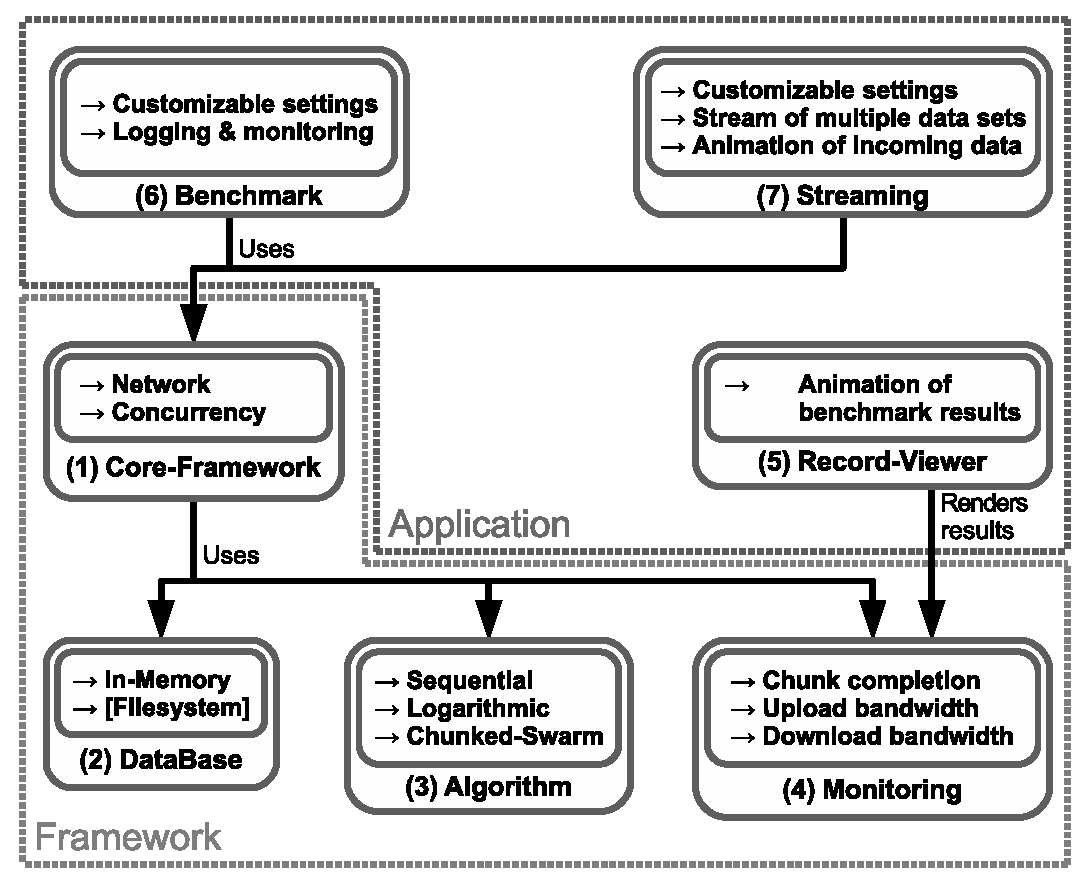
\includegraphics[width=0.8\linewidth]{arch}
	\caption{Software Architecture}
	\label{fig:arch}
\end{figure}

This chapter explains the architecture of the software in detail. From the beginning, one of the main goals were to achieve high modularity, so individual parts can be enhanced or replaced easily. The software is separated into the framework and the application part, which consists of multiple modules. Figure \ref{fig:arch} shows the architecture. 

\vfill
\pagebreak

The application part depends on the Core-Framework and the Monitoring module. It contains three modules which are Benchmark, Streaming and Record-Viewer. The Benchmark module is the most important application part, because it can help to create, monitor and evaluate different scenarios in terms of performance and efficiency. All measurements were done using this module. The Streaming module demonstrates the possibility for an incremental stream of data sets. The Record-Viewer module can render and animate results taken from the Monitoring module, which belongs to the framework part and thus only depends on it.

The Core-Framework, DataBase, Algorithm and Monitoring module are framework modules. While the DataBase, Algorithm and Monitoring module can be replaced or even omitted the Core-Framework module is fundamental. It manages network, concurrency and the communication of the three other modules located in the framework part. The DataBase module represents an interface for a generic data storage, which might be the file system or even completely in-memory. The Algorithm module contains the implementations of the concepts presented in Chapter \ref{theory}. To implement and test new distribution algorithms only this module has to be modified. The Monitoring module records data like current bandwidth usage and chunk completion, which are important data for evaluating the distribution algorithms. This module creates \emph{CSV} files, which can be plotted with tools like \emph{GNUplot}\footnote{http://www.gnuplot.info} and a log file, which contains a chronological stream of events occured during the recording and can be rendered using the Record-Viewer module.

In the next chapters the framework and application modules are explained in detail. The order is bottom-up, which means the Core-Framework module is explained first in Chapter \ref{module:core} followed by the DataBase and Algorithm in Chapter \ref{module:database} and \ref{module:algorithm} respectively. The Monitoring, Record-Viewer and Benchmark modules are discussed together in Chapter \ref{module:monitoring}. Lastly, the Streaming module is presented in Chapter \ref{module:streaming}.
\cleardoublepage
%!TEX root = bachelor.tex

\chapter{Modules}
\label{module}

\section{Core-Framework}
\label{module:core}

\subsection{Network}
\label{module:core:net}
The network implementation uses the concept of \emph{leechers} and \emph{seeders}. A leecher connects to one or more seeders and downloads chunks from them. A seeder has multiple leechers connected to it and uploads chunks to them. Chunk transfers are pull-based, so they can only be requested by the leecher, while meta data or address announcements are push-based and thus transferred without being requested. Therefore, every leecher knows exactly what a seeder has to offer without asking, but only requests the chunks it needs. See Section \ref{module:core:net:downloadreq} for more information.

While leechers and seeders are independent of each other, it is possible to couple them together. A leecher coupled with a seeder always announces the address of its seeder to any other seeder it is connected with. This concept is explained in more detail in Section \ref{module:core:net:autoconnect}.

Both, a leecher and a seeder, keep a reference to a database instance. A leecher stores downloaded data in its database and a seeder uploads data from its database. It is possible that both reference the same database instance, so the seeder is able to upload data, which was downloaded by the leecher. The DataBase module and all related concepts are explained in Section \ref{module:database}.

Leechers and seeders are associated with one of the multiple distribution algorithms defined in the Algorithm module. These algorithms determine the distribution behavior, which is further described in Section \ref{module:algorithm}.


\subsubsection{Automatic Connect}
\label{module:core:net:autoconnect}




\begin{figure}[ht]
	\begin{center}
		\subfigure[Seeder Discovery\label{fig:autoconnect}]{
	 		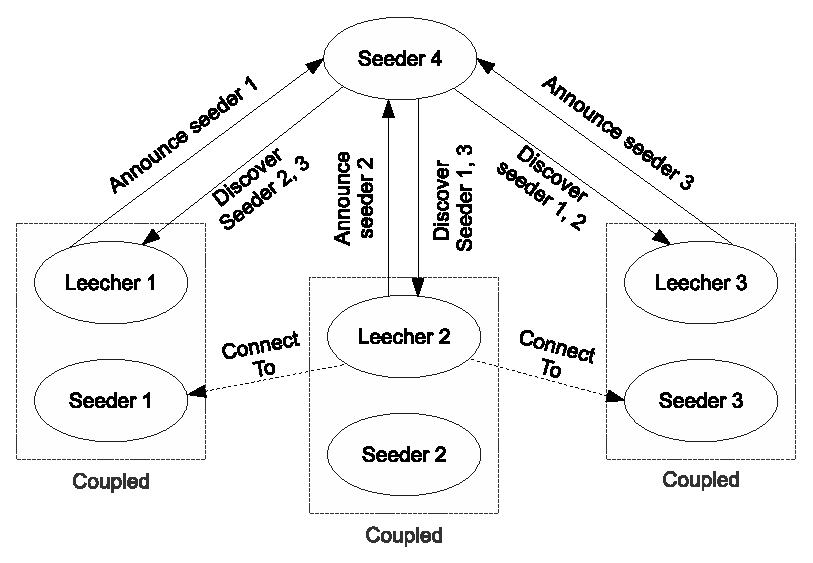
\includegraphics[width=0.6\textwidth]{autoconnect}
	 	}

		\subfigure[Reconnect\label{fig:reconnect}]{
	 		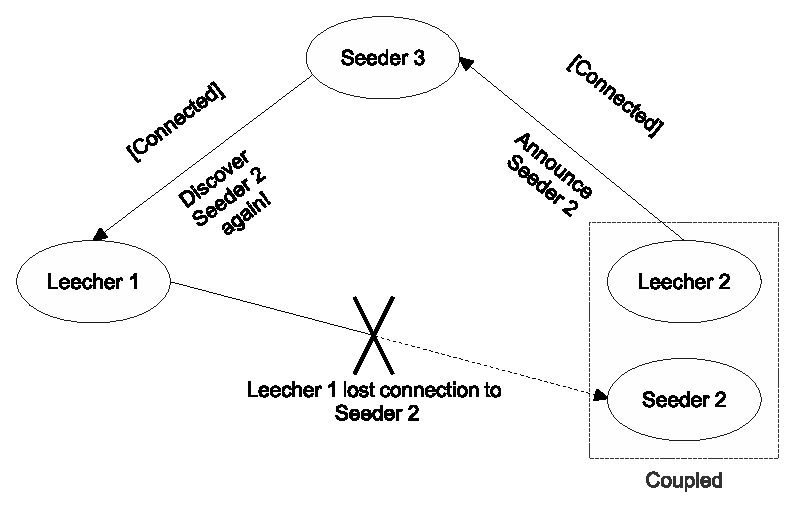
\includegraphics[width=0.6\textwidth]{reconnect}
	 	}~ % No whitespace here!
	 	\subfigure[Leecher\,/\,Seeder Mesh\label{fig:mesh}]{
	 		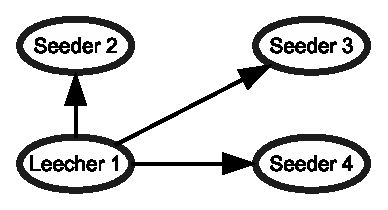
\includegraphics[width=0.25\textwidth]{mesh}
	 	}

		\caption{Automatic Connect}
	\end{center}
\end{figure}


Figure \ref{fig:autoconnect} shows in detail how the automatic connect mechanism works. Every leecher has to manually connect to a seeder for the first time, thereafter a leecher is able to automatically connect to other seeders. In order to provide this functionality every leecher, who is coupled with a seeder, announces the address of its coupled seeder to all other seeders it is currently connected with.

In this scenario leechers one, two and three announce the addresses of their seeders to seeder four, which broadcasts these addresses to all connected leechers. This way the leechers get to know each other and can connect to the remaining seeders. In figure \ref{fig:autoconnect} only the new connections of leecher two are illustrated, though leecher one and three connect to the other seeders as well. This works recursively, so if one of the seeders already has other leechers connected to it, these also will be found. Finally, the topology is just a mesh with $(n\:-\:1)\cdot n$ connections, where $n$ refers to the total number of coupled seeders and leechers and every leecher of each couple is connected to every seeder of all other couples. Figure \ref{fig:mesh} shows this from the point of view of leecher two, which is connected to all others seeders.

The mesh topology implies, that every peer knows exactly, what data sets other peers have and thus can request chunks efficiently, though it adds exponentially growing overhead and thus does not scale indefinitely. To improve scalability, the number of connections per leecher can be limited, which also limits the knowledge of each leecher and thus the ability to make good decisions what to request from whom.

If a leecher loses, for some reason, the connection to a seeder, the framework is able to reconnect, if the seeder is still online. This will be detected by periodic address broadcasts. So if, as shown in figure \ref{fig:reconnect}, leecher one lost the connection to seeder two but leecher one and two are also connected to seeder three, then seeder three will notify leecher one, that seeder two still exists.


\subsubsection{Meta Data Announcements}
After a leecher connected to a seeder, the leecher does not know, which data sets the seeder offers. As previously explained in Section \ref{module:core:net:autoconnect}, leechers discover new seeders through seeders they are already connected with. The way a leecher collects knowledge about the data sets a seeder offers works in a similar way. A seeder announces periodically its data sets to all connected leechers. It basically transfers a list of meta data, which is explained further in Section \ref{module:database:metadata}, so every leecher can update its knowledge about this seeder. The list of meta data can be modified by the used distribution algorithm before it is announced to model a specific distribution behavior. Section \ref{module:algorithm} outlines this mechanism.

An optimization uses a lazy transmission approach, thus a seeder will only transfer meta data, if it has changed. So if a data set does not change at all, a seeder will never transfer a second announcement of this data set. Another optimization causes the seeder not to transfer any announcements to leechers, which the seeder is uploading data to. This feature is further explained in the following Section \ref{module:core:net:downloadreq}.


\subsubsection{Download Requests}
\label{module:core:net:downloadreq}
After a leecher successfully connected to one or more seeders and has already received meta data announcements, it can start to request chunks from the seeders. What to request from whom heavily depends on the used distribution algorithm, which is explained in Section \ref{module:algorithm} in more detail. 

Since downloading more than one chunk at a time from the same seeder is not faster than downloading them sequentially, only one download per seeder at a time is allowed, which also reduces protocol complexity. Because of that, during a chunk download meta data and address announcements are not transferred, because these are obviously of no interest for the leecher. As soon as the chunk download completes, outstanding announcements will be bundled and transferred.

A seeder is allowed to decide whether a chunk request is valid or not, which means depending on the algorithm the seeder can reject a chunk request. If a seeder rejects a chunk request the leecher will not request the same chunk again. The seeder can tell the leecher, that a previously rejected chunk request is valid again by reannouncing this specific chunk. This way complex distribution behavior
can easily be implemented.


\subsubsection{Nonblocking I/O}
Network communication is based on \emph{sockets}, which can either be datagram or stream based. Datagram sockets are connectionless, so they are of no importance for this thesis. Instead, the network implementation uses stream sockets. A stream socket is always connected to another socket. Programmatically, these two sockets behave like files. If data is written to a socket, it will be transferred to the other socket and can be read from it then. As with files, socket operations usually block the currently executing \emph{thread} until the requested data is read or written, so this requires one thread per socket to handle multiple sockets concurrently. Unfortunately, threads are a limited resource, because they increase memory and \emph{CPU} usage. Therefore, this concept does not scale well.

To handle multiple sockets per thread, so called \emph{nonblocking} sockets in combination with \emph{event-polling} can be used. A nonblocking socket generally does not block on an operation, but returns an error instead, if it is not ready to execute this operation immediately. In combination with event-polling a thread can listen on sockets and be notified when these are ready. With this technique a single thread can handle tens of thousands of sockets.

Unfortunately, nonblocking sockets increase the complexity significantly, so the network implementation uses a framework to simplify the usage of them. The framework is called \emph{Netty 5} and written in Java. Netty supports the separation of the transport protocol and the logic, so underlying transport protocols, like \emph{In-VM}, \emph{TCP}, \emph{SCTP} or \emph{UDT}, can be changed without affecting the logic of the application. By default, only In-VM and TCP is used, which are explained in Section \ref{module:core:net:transport}.

\subsubsection{Transport: In-VM and TCP}
\label{module:core:net:transport}
Netty offers an In-VM, also called local, transport protocol, which does not involve network at all. It only works inside a single instance of the \emph{JVM} and is perfectly suited for simulations or benchmarking. This is because, the local transport does not require (de-)serialization of data, which eliminates a huge amount of memory and CPU usage. Normally, the overhead of serialization is negligible, but the Benchmark module is able to simulate a large number of seeders and leechers, so these overheads can sum up to a significant number. Therefore, the local transport seems to be the perfect fit for this purpose.

Netty also offers common transport protocols like TCP. It is used as a secondary option for the Benchmark module, which is useful to run distributed benchmarks on multiple machines, because local transport is limited to a single JVM instance.


\subsubsection{Traffic-Shaping}
In order to simulate and evaluate network applications, the ability to control the bandwidth to have comparable network conditions is needed. The problem with bandwidth limitation, which is also called traffic-shaping, is that the writer can not be throttled. The writer can either write as fast as possible or not write at all. In order to limit the bandwidth, the writer has to be started and stopped periodically. Since readers and writers are identical in terms of bandwidth limitation, the explanation always refers to writers but the same approach works for readers equally well.

If the limitation period is too long, the introduced bandwidth peaks will affect the measurements in a negative way, but if the period is too short instead, overhead will be increased. To perfectly limit the bandwidth an indefinitely short interval is needed. So, if the traffic-shaping shall work reliably the sweet spot between accuracy and minimal overhead has to be found. The network implementation uses a period of 250\,ms, which offers enough precision, because the measurements are done every second. So every measurement contains the average of approximately four bandwidth limitation runs.

The complexity increases using multiple writers, who are not allowed to exceed a shared bandwidth. The main problem is fairness. It is not desired, that one writer gets 95\,\%, while the remaining writers share only 5\,\% of the bandwidth. At the same time a single writer should be able to write at full speed, when no one else is writing. This complex behavior can be achieved using a \emph{leaky-bucket} algorithm and a \emph{priority-queue}.

A leaky-bucket contains tokens, where a token equals one byte. If a writer wants to write a message, it will try to remove the tokens needed for the message to transfer. If the bucket does not have enough tokens, the writer will take the remaining tokens and will decrease the size of the message it wants to write by the number of removed tokens. After this, the writer waits until the bucket gets refilled and repeats the procedure. Unfortunately, this does not fix the fairness problem.

To solve the fairness problem a writer is not allowed to remove tokens from the bucket directly. Instead it inserts the write request into a priority-queue. A writer job constantly polls the head of the queue and tries to process the write requests using the leaky-bucket. This time, the writer increases its number of written bytes according to the size of the written message. If the writer has more messages to write, it will insert itself into the queue according to the number of total written bytes compared to other writers. This way the head of the queue always is a write request belonging to a writer, which has written the fewest number of bytes in total. Thereby we get good fairness with almost no overhead, because the writer job runs only on demand in a thread pool and quits after all write requests are processed.


\subsection{Concurrency}
With the use of nonblocking sockets it is possible to handle a lot of sockets with only one thread. But this can be further improved, because modern CPUs always have multiple cores, whose quantity determines the number of threads able to run in parallel. For example, if a CPU has four cores and the application only uses one thread, the CPU will be utilized by only 25\,\%. Wherefore Netty uses more than one thread to increase the efficiency. In the next Section \ref{module:core:conc:eventloop} the utilization of multiple threads is explained in more detail.

\subsubsection{Event-Loop}
\label{module:core:conc:eventloop}
Netty has the notion of an \emph{event loop}. An event loop is always running in its own thread and processes queued events one after the other. These events are mostly readiness events notifying a given socket is now readable, writable, acceptable or connectable.

To use more than one thread, Netty simply spawns more event loops, typically just as many as there are CPU cores. New sockets will then be distributed evenly among all running event loops. Even if the event loops get unbalanced, Netty will try to rearrange the sockets so that the event loops become balanced again.

These event loops can then run theoretically in parallel, because the underlying operating system distributes busy threads equally among all available cores. But using more than one thread is only the tip of the iceberg, multiple threads introduce a whole new category of problems and considerations, which have to be taken into account. The next Section \ref{module:core:conc:lockfree} discusses this a bit more in depth.


\subsubsection{Lock-Free Progamming}
\label{module:core:conc:lockfree}
The main problem using multiple threads is the question of how these threads interact which each other. If two threads access the same variable without any protection, the resulting behaviour is not always defined and can lead to untraceable bugs. The unprotected access of variables is called a \emph{race condition} or \emph{critical-section}.

A simple solution is to protect those sections with a mutually exclusive (mutex) lock, which simply forbids that more than one thread is entering the critical section at a time, but this decreases efficiency and increase thread context switching, which is expensive. One solution is to use lock-free algorithms, which exploit certain guarantees made by the Java memory model. The in-depth explanation of these concepts would arguably exceed the boundaries of this thesis, but it should be noted, that the network implementation heavily uses those algorithms.

The reason why those concepts were considered is that inter-thread communication was a key design choice in order to simplify the architecture of the implementation. For instance a leecher can be connected to a lot of seeders receiving a lot of meta data and address announcements. In order to effectively request chunks from the seeders, the leecher has to collect the information from all connections, which may run in different event loop threads and thus are not protected against concurrent access by default. Since this collection is a common task, it should be optimized as well. Using so called \emph{compare and swap (CAS)} and volatile operations the necessary mutexes can be reduced to a minimum. 

Usually, the overhead of mutexes can be ignored, but the simulation of hundreds of leechers and seeders on multiple cores means a lot of cross thread access. If every collection of meta data of each leecher would stop all event loop threads by using a mutex, the overhead should start to be noticeable. These impacts are hard to measure or quantify, though. But in principle the lock-free approach scales better. As a rule of thumb lock-free algorithms should always be preferred in performance critical sections. They can also help to prevent \emph{dead locks}, which happen when two threads are waiting for resources locked by each other, and thus both wait forever.


\section{DataBase}
\label{module:database}
The DataBase module represents a generic interface for storing binary data sets as chunks in any kind of storage. It has the responsibility to verify written chunks in terms of consistency and validation. But to do so the database has to know about the structure of the data set. Therefore, the meta data, which describes a given data set, is stored together with the data set as key-value pairs. The next Section \ref{module:database:metadata} describes the meta data format in more detail.


\subsection{Meta Data}
\label{module:database:metadata}
The meta data contains information about a given data set. These information are transferred between seeders and leechers to describe what data sets are available, and thus which chunks can be requested. The following information are stored in the meta data: \emph{Name}, \emph{Description}, \emph{ID}, \emph{Size}, \emph{Chunks}, \emph{Hash} and \emph{ChunkedHashes}.

The Name and Description fields are used for human related tasks. The ID is used for streaming purposes, which will be explained later in Section \ref{module:streaming}. The Size field determines the total size of the data set including all chunks, which leads to the next field. The Chunks field is a bit set, which simply stores one or zero bits for existing or missing chunks respectively. The length of the bit set determines the number of chunks a data set has. The Hash field contains a checksum generated by a hash algorithm like \emph{SHA-1} from the whole data set. The ChunkHashes field does the same but for each chunk individually. This way the database can verify single chunks as well as the data set in total. The reason why there is an extra Hash field for the whole data set is to reduce the chance of hash collision. Two data sets are considered equal if all of their fields are equal as well.


\subsection{Backends: Emulated, In-Memory and Persistent}
\label{module:database:backend}
The emulated backend does not store any data sets directly. Instead, it only stores which data sets and chunks are available and thus causes no overhead at all. If data sets are queried, empty buffers are returned. The in-memory backend stores data sets in main memory and is not persistent. It is a useful backend for situations, where data sets are generated or consumed on the fly like video streaming or test scenarios. In case of video streaming, a webcam could act as a data set source and thus chunks are transmitted directly from it. This backend has almost no overhead other than memory usage. The persistent backend implements a database based on a file system, which can also be virtual like a \emph{ZIP} file. This backend is more rigid but also very important for file sharing applications.



\section{Algorithm}
\label{module:algorithm}
This module contains the algorithms which determine the distribution behavior. While the Core-Framework module takes care of all the low-level parts the computing work is done here. This module defines two interfaces for both, a seeder and a leecher, which are called \emph{SeederDistributionAlgorithm} and \emph{LeecherDistributionAlgorithm} respectively. 

A SeederDistributionAlgorithm can modify meta data, which is announced by a seeder and allows or rejects chunk requests. A LeecherDistributionAlgorithm is even simpler, it can only request chunks. A schematic representation of both interfaces looks like this:

\begin{verbatim}
interface SeederDistributionAlgorithm {
    List of MetaData modifyMetaData(List of MetaData)
    Bool isChunkRequestAllowed(ChunkRequest)
}

interface LeecherDistributionAlgorithm {
    List of ChunkRequest requestChunks(AvailableDataSetsOfAllSeeders)
}
\end{verbatim}

These interfaces are totally independent of the underlying network implementation. As a core concept, a leecher algorithm is only interested in requesting chunks as efficient as possible. The seeder can decide if a requested chunk request is allowed or not and what meta data it announces. With these two methods a seeder can model the behavior of a seeder which uploads to every leecher in parallel, or only to one leecher in total, or even stop announcing meta data, if the associated data sets have already been transferred, which is used by the Chunked-Swarm model and explained in Section \ref{module:algorithm:chunkedswarm}. In the next sections all implemented distribution algorithms are compared and explained in detail.

\subsection{Algorithms: Sequential and Logarithmic}
\label{module:algorithm:seqlog}
The Sequential and Logarithmic model, explained in Section \ref{theory:model:sequential} and \ref{theory:model:logarithmic} respectively, both share the same LeecherDistributionAlgorithm, which is the \emph{OrderedSingleMostLeecherDistributionAlgorithm}. This algorithm chooses a seeder, which has the complete data set and requests it from this seeder. It does only work with a chunk count of one and never requests a data set from more than one seeder in parallel.

For seeding the Sequential model uses the \emph{DefaultSeederDistributionAlgorithm}, which uploads data sets to every leecher asking for one. It is important to note, that this model has only one seeder and many leechers. All leechers are connected to this seeder and download data sets sequentially. 

The Logarithmic model is fundamentally different in this regard, because every peer has a leecher coupled with a seeder and is connected to every other seeder of the network. This model uses the \emph{LimitedSeederDistributionAlgorithm} for seeding and uploads data sets only to one leecher in parallel. During an upload other requests are rejected. The meta data of data sets which are being uploaded are also removed from the meta data announcement set, so new leechers will not request these data sets. After an upload is complete, the meta data of the particular data set is announced again.

\subsection{Algorithm: Chunked-Swarm}
\label{module:algorithm:chunkedswarm}
The Chunked-Swarm model, which is presented in Section \ref{theory:model:chunkedswarm}, allows multiple uploads in parallel and requires a chunk count equal to or greater than the number of peers. Every seeder uses the DefaultSeederDistributionAlgorithm and thus uploads chunks to every leecher. The leechers use the \emph{OrderedChunkedSwarmLeecherDistributionAlgorithm}, which is similar to the OrderedSingleMostLeecherDistributionAlgorithm, but requests single chunks instead of complete data sets and will download from any seeder the leecher is connected with in parallel, if possible. 

To effectively download from as many seeders as possible, all seeders are sorted by the number of chunks they offer in ascending order, but without the chunks, which are currently being downloaded by the leecher and those, which are already downloaded. The leecher then traverses the sorted list of chunks and requests one chunk from each seeder. After each request the list is sorted and filtered again, so that the chunk the leecher just requested is not requested from another seeder as well. 

This way the leecher always chooses the best combination of chunk requests. If there are multiple chunks per seeder, which are equally well suited for downloading, the algorithm picks one chunk randomly. In consequence of this, chunk duplication can not be prevented, though minimized, if a high chunk count is chosen. Although, the efficiency of this model was determined with perfect chunk selection in mind. 

Since random chunk selection can not always be perfect, an additional so called \emph{SuperSeederDistributionAlgorithm} can be chosen. It is basically a DefaultSeederDistributionAlgorithm which remembers all chunks it has already uploaded and rejects any further attempts to download these chunks. It is typically used by only one seeder in the network, which is then called a \emph{super seeder}. This way chunk duplication can not occur, because leechers, whose chunk requests are rejected, simply request another chunk and request the rejected chunk later from normal seeders. The method guarantees that every leecher requests a distinct chunk from the super seeder, which has the complete data set at the beginning. The other seeders still use the DefaultSeederDistributionAlgorithm. The problem is, that this technique is not safe against peer loss, which means that chunks uploaded to a peer, which goes offline, are not retransferred by the super seeder by default. This relates to future work and could be solved by periodic checks, which determine whether a peer is still online.


\section{Monitoring, Record-Viewer and Benchmark}
\label{module:monitoring}

To measure the quality and efficiency of the framework, the Monitoring module collects data like current bandwidth usage, total transferred bytes and chunk\,/\,data set completion timestamps from every peer. The current upload bandwidth usage and total uploaded bytes are only collected from seeders, while the current download bandwidth usage and total downloaded bytes are only collected from leechers. The reason for this is that leechers upload almost nothing, they only announce the address of their coupled seeder once and upload a chunk request for each chunk. These chunk requests are very small and usually only transferred once every few seconds, depending on the chunk size. In consequence of that, the seeders only download these address announcements and chunk requests from their leechers, so seeders download almost nothing as well.

The collected data is then stored in csv files, which contain columns for every leecher and\,/\,or seeder, depending on the collected data. Because these sole files are not very meaningful, a small collection of python scripts help to manage them. For instance, if there are multiple csv file sets from many runs, the merge script can calculate the mean and the confidence interval of all runs. Also, additional csv files are created from existing csv files, like the SortedTotalUploadedBandwidth.csv and SortedChunkCompletion.csv files which are, as the name let assume, sorted. In case of the SortedTotalUploadedBandwidth.csv file, the entries are sorted by the amount of uploaded bytes and the SortedChunkCompletion.file is sorted by the time needed to complete all chunks\,/\,data sets. Both files are sorted in descending order.

Besides the csv files, the Monitoring module can create a log file, which contains a chronological stream of events occurred during a run. Amongst others, these events are chunk requests, starts of uploads and downloads and chunk\,/\,data set completions. The content of the log file can be rendered using the Record-Viewer module. Those events are stored using Java serialization and could be generated by the Benchmark module or any other application, which uses the Monitoring module.

The Benchmark module consists of a command line application, which simulates a configurable number of seeders and leechers in one process and records its runtime behavior. The application can be configured in several ways to implement a wide range of scenarios and is bundled as a Java archive (\,\emph{jar}\,) file. This module uses the emulated database backend, which is explain in Section \ref{module:database:backend}, so there is almost no overhead involved.


\section{Streaming}
\label{module:streaming}

The Streaming module contains an experimental implementation of a video streaming server, where peers can start watching a video file roughly at the same time and continue watching the video while they are downloading and distributing new chunks from the server. 

In order to transfer the data set to all peers continuously, the video file has to be separated into multiple parts, which consist of multiple chunks. Programmatically, each part is represented by a data set, so there does not exist a data set describing the whole video file. To determine which data set represents which part of the video file, the meta data of each data set contains an ID field, which is linearly incremented for each part. All data sets combined together represent the whole video file. The peers always try to download and distribute data sets with the smallest ID field. This way, the video file is distributed sequentially while retaining the efficiency of the Chunked-Swarm model.

The size of the parts have to be chosen wisely, because it determines how long it takes to distribute a part among all peers. Peers can only start watching the video, when there is at least one part available, so the size of the parts directly affects the quality of service. The correct choice of the size also depends on the number of chunks and thus on the number of peers.

The Streaming module uses a \emph{HTTP} server to deliver the data sets from the database as a video stream. Even if there is only one data set available, the HTTP server will set the content length of the HTTP response to the length the of the whole video file. Therefore, external video players can simply play the whole video file at once. If the video player requests a position in the video stream, which is not available yet, the HTTP server will wait until the database contains enough data sets to process the request. From the point of view of the video player it looks like the data arrives very slowly and thus waits until enough bytes have been buffered to play the video fluently.

\cleardoublepage
%!TEX root = bachelor.tex

\chapter{Evaluation}
\label{evaluation}

This chapter contains the evaluation of the framework. It starts with expectations and the used methodology in Section \ref{evaluation:expectations}. Then, different scenarios are described and evaluated in Section \ref{evaluation:1}, \ref{evaluation:2}, \ref{evaluation:3}. \ref{evaluation:456}, \ref{evaluation:78910} and \ref{evaluation:1112}.

\section{Expectations and Methodology}
\label{evaluation:expectations}

The efficiency of the different distribution models is already discussed theoretically in Chapter \ref{theory}. While the trade-offs are already known, the implementation of these models can cause unexpected side effects, which could have an impact on performance. The main goal of this evaluation is to verify, that the implementation of the Chunked-Swarm model is able to keep the $2\:T_0$ limit in practice, as predicted in Section \ref{theory:model:chunkedswarm}.

Therefore, the Benchmark module is used to simulate certain scenarios and thus to measure the influence of certain parameters like number of peers, upload and download bandwidth, chunk count and so on. The Monitoring module, see Section \ref{module:monitoring}, is used to record the current upload and download bandwidth and completion time of each peer during the benchmarks.

In order to get meaningful results, every scenario using the Chunked-Swarm model runs ten times, except those, which use the Sequential and Logarithmic model, because these models behave always predictable. In case of scenarios using the Chunked-Swarm model, the results are merged by calculating the mean and the confidence interval using a condidence level of 95\,\% of all runs. All results are plotted using gnuplot.

There are twelve scenarios in total. The first scenario is considered the default, while the remaining scenarios are variations of it. To measure the influence of each parameter, the scenarios have always only one parameter, that is different to the default scenario. All scenarios run on a virtual server with 14 \emph{Intel Xeon} 2.1 Ghz cores and 38 GB main memory.

\begin{figure}[!ht]
	\begin{center}	
		\subfigure[Completion Process\label{fig:s1:completion}]{
	 		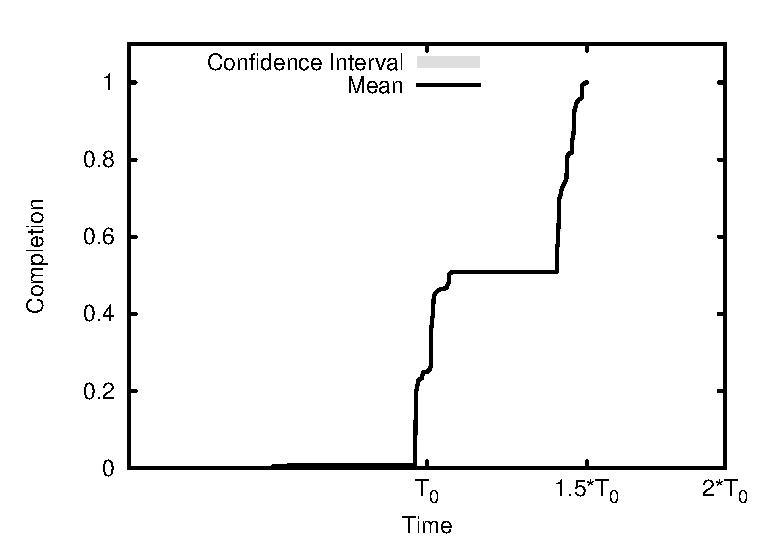
\includegraphics[width=0.5\textwidth]{plots/scenario_1_default/plots/GeneratedMeanChunkCompletion.csv}
	 	}~ % No whitespace here!
	 	\subfigure[Sorted Completion\label{fig:s1:scompletion}]{
	 		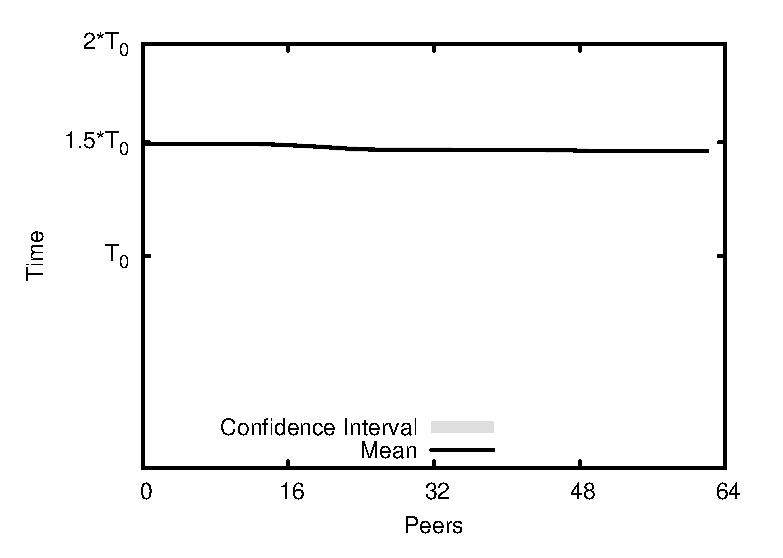
\includegraphics[width=0.5\textwidth]{plots/scenario_1_default/plots/GeneratedMeanSortedChunkCompletion.csv}
	 	}		

	 	\subfigure[Super Seeder Upload Bandwidth\label{fig:s1:ssupload}]{
	 		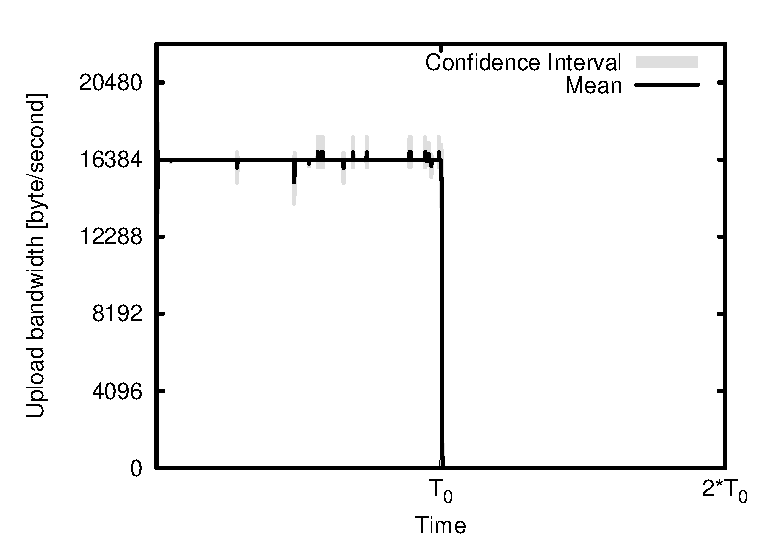
\includegraphics[width=0.5\textwidth]{plots/scenario_1_default/plots/GeneratedMeanCurrentSuperSeederUploadBandwidth.csv}
	 	}~ % No whitespace here!
	 	\subfigure[Seeder Upload Bandwidth\label{fig:s1:upload}]{
	 		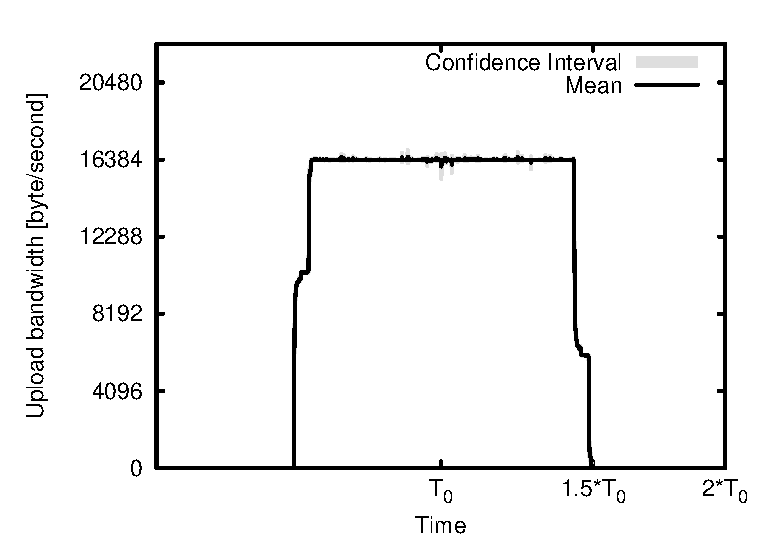
\includegraphics[width=0.5\textwidth]{plots/scenario_1_default/plots/GeneratedMeanCurrentUploadBandwidth.csv}
	 	}

	 	\subfigure[Leecher Download Bandwidth\label{fig:s1:download}]{
	 		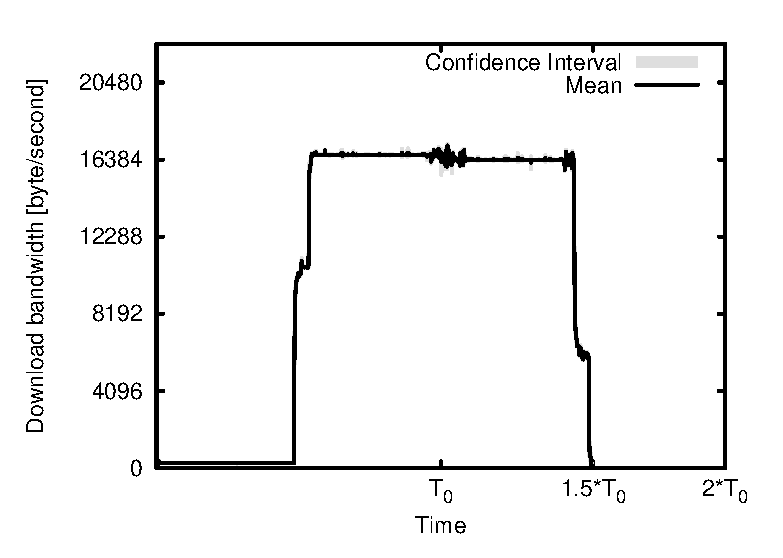
\includegraphics[width=0.5\textwidth]{plots/scenario_1_default/plots/GeneratedMeanCurrentDownloadBandwidth.csv}
	 	}
		\caption{Scenario 1 - Default}
		\label{fig:s1}
	\end{center}
\end{figure}


\section{Scenario 1: Default}
\label{evaluation:1}

Scenario 1 simulates 64 peers using the Chunked-Swarm model, as explained in Section \ref{theory:model:chunkedswarm}, with super seeder extension, see Section \ref{module:algorithm:chunkedswarm}, where one peer has the complete data set at the beginning, which is called the super seeder and does only upload each chunk once. Every peer has a simulated upload bandwidth of $16.384\:\frac{bytes}{seconds}$. The download bandwidth is not limited. The size of the data set is not specified directly, but is calculated from the upload bandwidth and $T_0$, which is set to ten minutes (600 seconds). So a single transfer from the super seeder to one peer takes exactly $T_0$ seconds. The small upload bandwidth has a major advantage for benchmarking, because basically it represents the buffer size of each peer. So $n\:*\:u$ is the minimal memory usage of a benchmark, where $n$ is the number of peers and $u$ the upload bandwidth. If the upload bandwidth is too high, the overhead of the memory usage will influence the expressiveness of the benchmark. Since the size of the data set is always relative to the upload bandwidth and $T_0$, the actual upload bandwidth does not matter. The data set is also splitted into twice as many chunks as there are peers, but without the super seeder, which makes $63\:*\:2=126$ chunks. This scenario also simulates a meta data size of one byte. In reality, the meta data would be something about 64 bytes, because it contains a \emph{SHA-1} hash, a bit set and some network protocol headers, but because the upload bandwidth is reduced for the benchmark, the meta data size should be reduced as well. In this special case the $\frac{16.384\:\frac{bytes}{seconds}}{1\:byte}$ ratio is equal to $\frac{1.048.576\:\frac{bytes}{seconds}}{64\:bytes}$. So if we assume, that a usual peer has an upload bandwidth of $1.048.576\:\frac{bytes}{second}$, which is quite common these days, the benchmark values are realistic.

Figure \ref{fig:s1:completion} shows the mean completion graph for each peer, where the x-axis represents the time and the y-axis the completion of the data set from $0.0$ to $1.0$. After $1.5\:*\:T_0$ every peer has the complete data set available. As shown in Chapter \ref{theory}, the formula $T(n, c) = (1\:+\:\frac{n-1}{c})\:T_0$ calculates the time needed for the Chunked-Swarm model. So $c\:=126$, $n\:=\:63$ and $T(63, 126) = (1\:+\:\frac{63-1}{126})\:T_0 = 1,49\:T_0$. Figure \ref{fig:s1:scompletion} shows the mean completion time of all 63 peers, sorted in descending order. Since this graph is almost a horizontal line, all peers complete the transfer roughly at the same time.

Figure \ref{fig:s1:ssupload} shows the mean super seeder upload bandwidth. For $T_0$ seconds, the super seeder uploads at full speed after which it stops uploading, because the super seeder extension forbids uploading the same chunk twice, so every chunk is uploaded once. Figure \ref{fig:s1:upload} and Figure \ref{fig:s1:download} present the mean upload and download bandwidth of all remaining peers. Since there are twice as many chunks as peers, each peer can start uploading chunks after $0.5\:*\:T_0$ seconds, as described in Section \ref{theory:model:chunkedswarm}. It is important to note, that the super seeder and the remaining peers upload in parallel after $0.5\:*\:T_0$ seconds.



\begin{figure}[ht]
	\begin{center}
		\subfigure[Completion Process\label{fig:s2:completion}]{
	 		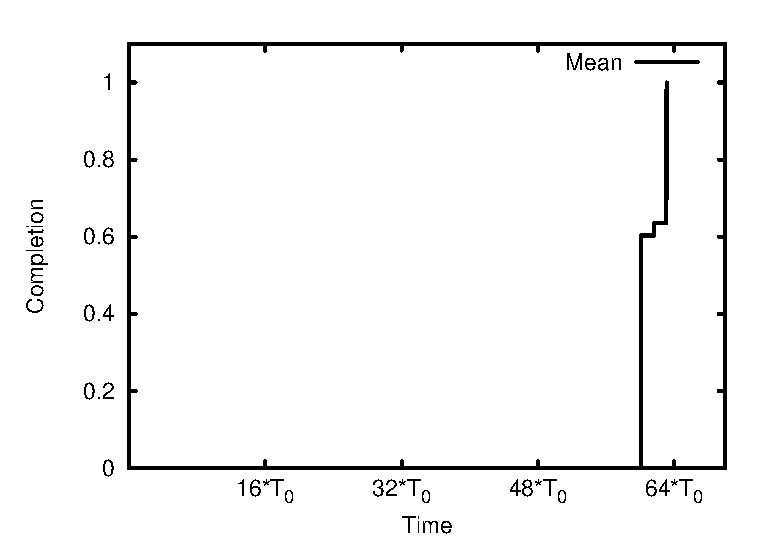
\includegraphics[width=0.5\textwidth]{plots/scenario_2_seq/plots/GeneratedMeanChunkCompletion.csv}
	 	}~ % No whitespace here!
	 	\subfigure[Sorted Completion\label{fig:s2:scompletion}]{
	 		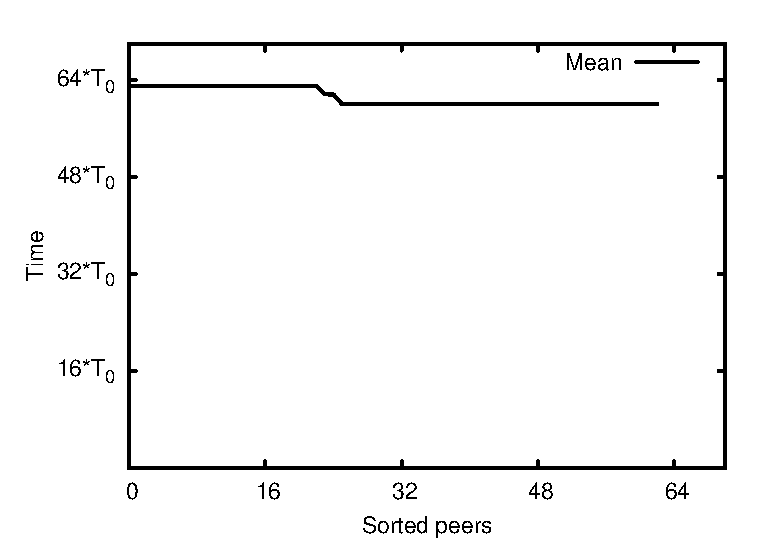
\includegraphics[width=0.5\textwidth]{plots/scenario_2_seq/plots/GeneratedMeanSortedChunkCompletion.csv}
	 	}	 	

		\subfigure[Leecher Download Bandwidth\label{fig:s2:download}]{
	 		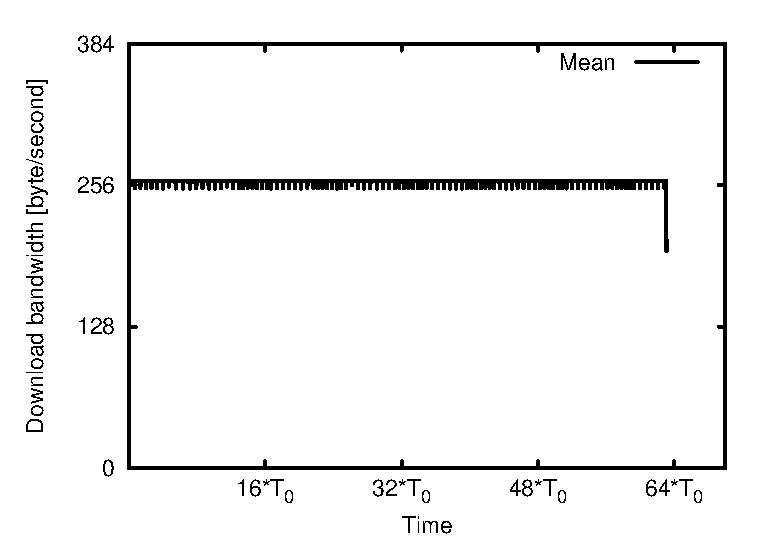
\includegraphics[width=0.5\textwidth]{plots/scenario_2_seq/plots/GeneratedMeanCurrentDownloadBandwidth.csv}
	 	}~ % No whitespace here!
	 	\subfigure[Super Seeder Upload Bandwidth\label{fig:s2:ssupload}]{
	 		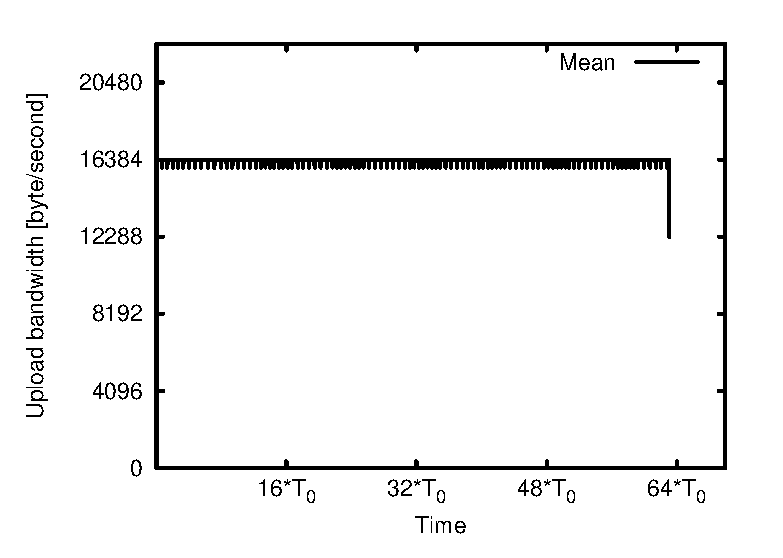
\includegraphics[width=0.5\textwidth]{plots/scenario_2_seq/plots/GeneratedMeanCurrentSuperSeederUploadBandwidth.csv}
	 	}

		\caption{Scenario 2 - Sequential}
		\label{fig:s2}
	\end{center}
\end{figure}

\pagebreak
\section{Scenario 2: Sequential}
\label{evaluation:2}

Scenario 2 uses the Sequential model, as explained in Section \ref{theory:model:sequential}, so there is only one seeder, which is uploading. This seeder is also called super seeder, though it is not related to the super seeder extension of the Chunked-Swarm model. This super seeder uploads data sets sequentially to all connected peers, which do not distribute these data sets among themselves. This scenario represents a client\,/\,server system, where the upload bandwidth is shared by all connected peers. All other parameters are taken from Scenario 1. As exptected, all peers need approximately $63\:*\:T_0$ seconds to complete the transfer, as shown in figure \ref{fig:s2:completion} and \ref{fig:s2:scompletion}. This makes sense, because every peer can only download with $\frac{16.384}{63}=267\:\frac{bytes}{second}$, while the super seeder uploads at full speed, see figure \ref{fig:s2:download} and \ref{fig:s2:ssupload}. The peaks in the upload and download bandwidth graphs are caused by the leaky-bucket algorithm used by the traffic shaping mechanism, see \ref{module:core:net:traffic}, and have no impact on performance.




\begin{figure}[!ht]
	\begin{center}	
		\subfigure[Completion Process\label{fig:s3:completion}]{
	 		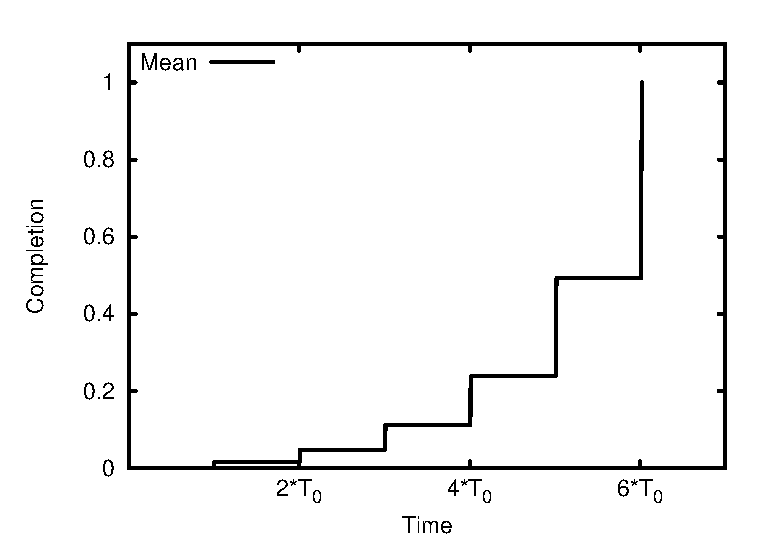
\includegraphics[width=0.5\textwidth]{plots/scenario_3_log/plots/GeneratedMeanChunkCompletion.csv}
	 	}~ % No whitespace here!
	 	\subfigure[Sorted Completion\label{fig:s3:scompletion}]{
	 		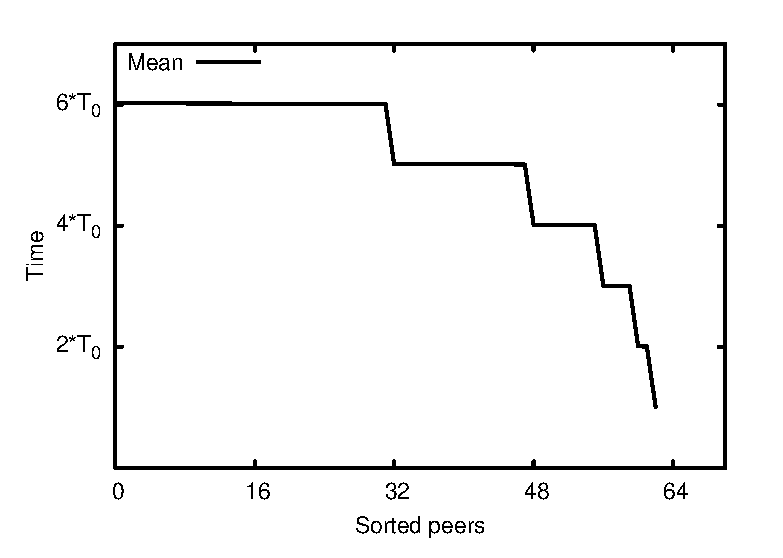
\includegraphics[width=0.5\textwidth]{plots/scenario_3_log/plots/GeneratedMeanSortedChunkCompletion.csv}
	 	}		

	 	\subfigure[Super Seeder Upload Bandwidth\label{fig:s3:ssupload}]{
	 		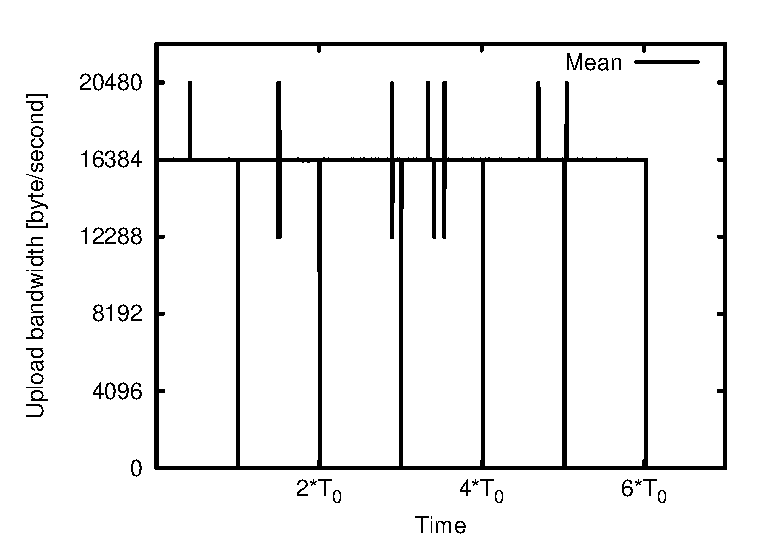
\includegraphics[width=0.5\textwidth]{plots/scenario_3_log/plots/GeneratedMeanCurrentSuperSeederUploadBandwidth.csv}
	 	}~ % No whitespace here!
	 	\subfigure[Seeder Upload Bandwidth\label{fig:s3:upload}]{
	 		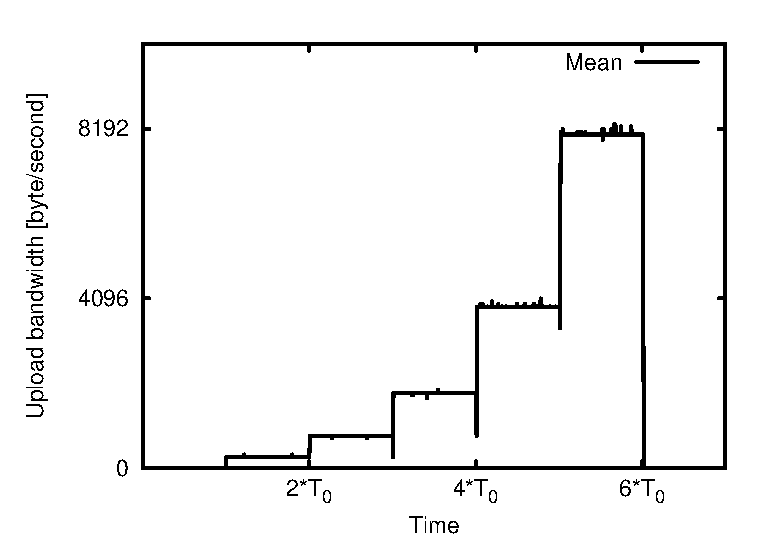
\includegraphics[width=0.5\textwidth]{plots/scenario_3_log/plots/GeneratedMeanCurrentUploadBandwidth.csv}
	 	}

	 	\subfigure[Leecher Download Bandwidth\label{fig:s3:download}]{
	 		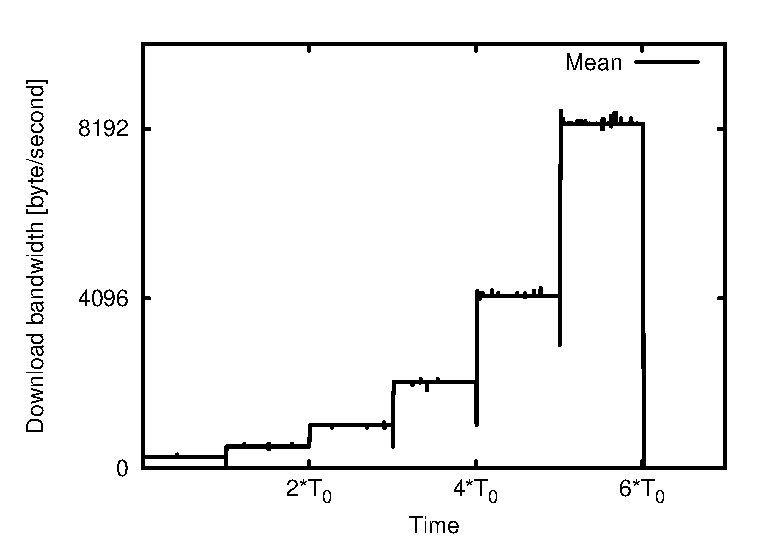
\includegraphics[width=0.5\textwidth]{plots/scenario_3_log/plots/GeneratedMeanCurrentDownloadBandwidth.csv}
	 	}
		\caption{Scenario 3 - Logarithmic}
		\label{fig:s3}
	\end{center}
\end{figure}

\pagebreak
\section{Scenario 3: Logarithmic}
\label{evaluation:3}

Scenario 3 uses the Logarithmic model. As explained in Section \ref{theory:model:logarithmic}, this model uses a Peer-to-Peer network, like the Chunked-Swarm model, but only complete data sets are tranferred and a single peer only uploads to one other peer in parallel. Only one peer has the complete data set at first, which is also called the super seeder. This way, the number of uploading peers doubles every $T_0$ seconds, so the number of uploading and completed peers grows exponentially, see figure \ref{fig:s3:completion} and \ref{fig:s3:scompletion}. But it also means, that there are never more than 50\,\% of all peers uploading in parallel, which is shown in figure \ref{fig:s3:upload} and \ref{fig:s3:download}. Figure \ref{fig:s3:ssupload} presents the super seeder upload bandwidth including some rough peaks, which are caused by the announce delay. When a peer completes a download, it takes a few seconds to notify the remaining peers in the network. During this time the super seeder is not uploading anything, so these peaks are actually expected. Like Scenario 2, the minor peaks are part of the traffic shaping mechansim.

\vfill


\pagebreak
\begin{figure}[!ht]
	\begin{center}	
		\subfigure[Completion Process\label{fig:s4:completion}]{
	 		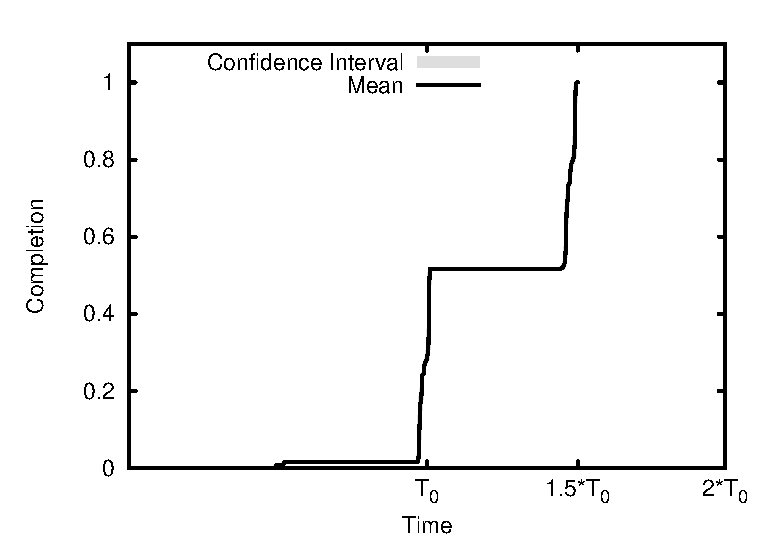
\includegraphics[width=0.5\textwidth]{plots/scenario_8_peer_count_32/plots/GeneratedMeanChunkCompletion.csv}
	 	}~ % No whitespace here!
	 	\subfigure[Sorted Completion\label{fig:s4:scompletion}]{
	 		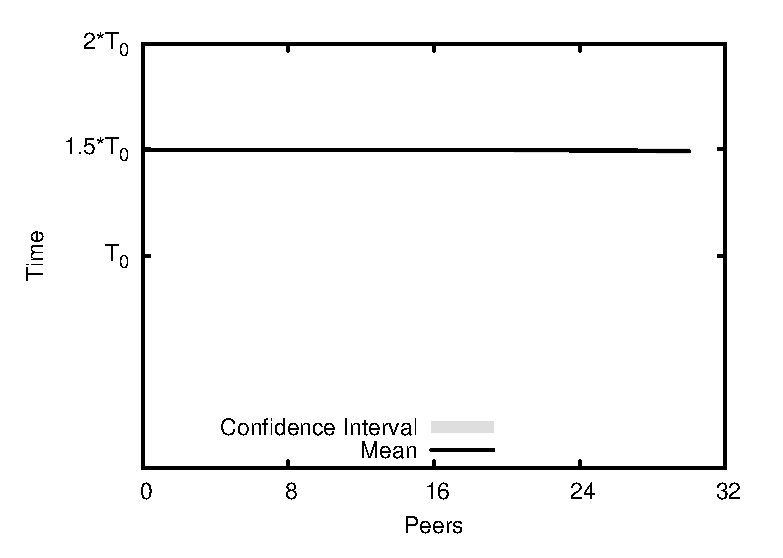
\includegraphics[width=0.5\textwidth]{plots/scenario_8_peer_count_32/plots/GeneratedMeanSortedChunkCompletion.csv}
	 	}		

	 	\subfigure[Super Seeder Upload Bandwidth\label{fig:s4:ssupload}]{
	 		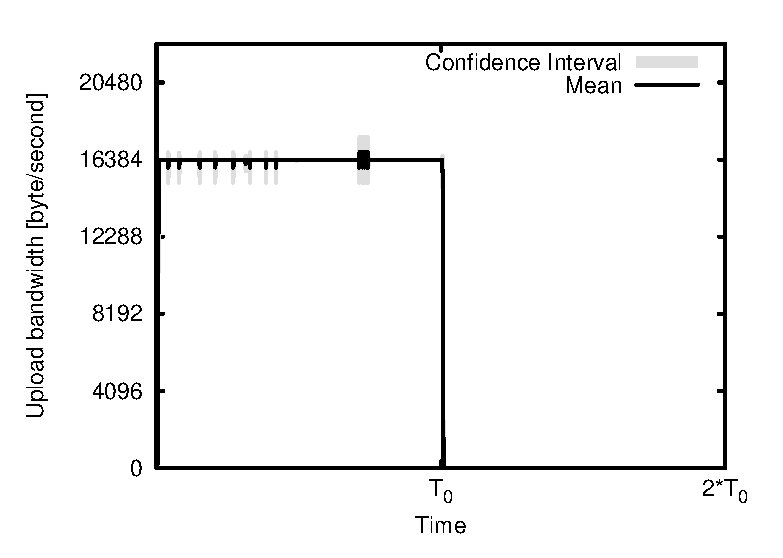
\includegraphics[width=0.5\textwidth]{plots/scenario_8_peer_count_32/plots/GeneratedMeanCurrentSuperSeederUploadBandwidth.csv}
	 	}~ % No whitespace here!
	 	\subfigure[Seeder Upload Bandwidth\label{fig:s4:upload}]{
	 		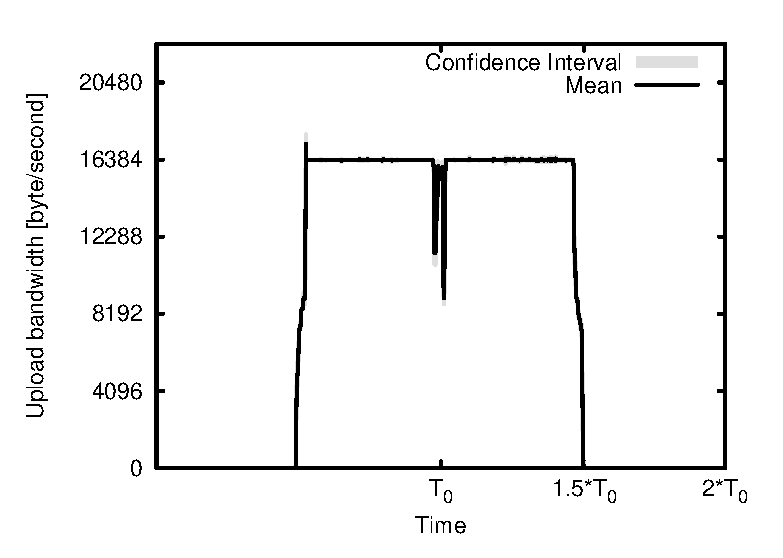
\includegraphics[width=0.5\textwidth]{plots/scenario_8_peer_count_32/plots/GeneratedMeanCurrentUploadBandwidth.csv}
	 	}

	 	\subfigure[Leecher Download Bandwidth\label{fig:s4:download}]{
	 		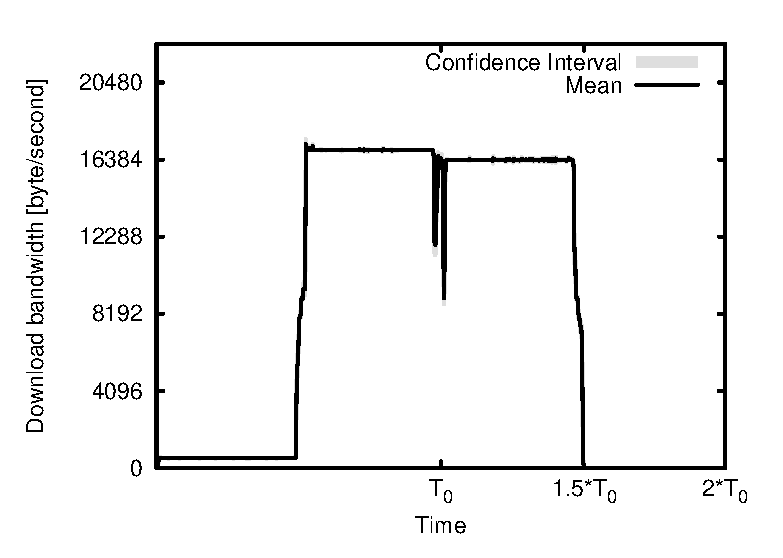
\includegraphics[width=0.5\textwidth]{plots/scenario_8_peer_count_32/plots/GeneratedMeanCurrentDownloadBandwidth.csv}
	 	}
		\caption{Scenario 4 - 32 Peers}
		\label{fig:s4}
	\end{center}
\end{figure}
\vfill

\pagebreak
\begin{figure}[!ht]
	\begin{center}	
		\subfigure[Completion Process\label{fig:s5:completion}]{
	 		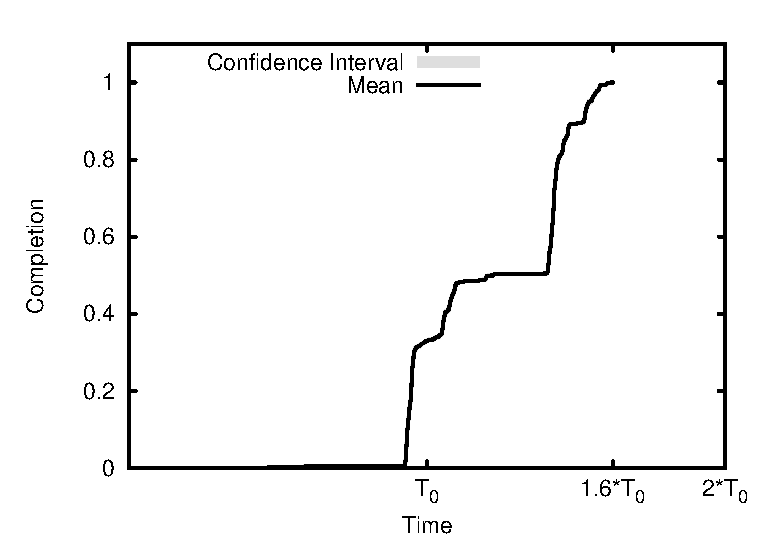
\includegraphics[width=0.5\textwidth]{plots/scenario_4_peer_count_128/plots/GeneratedMeanChunkCompletion.csv}
	 	}~ % No whitespace here!
	 	\subfigure[Sorted Completion\label{fig:s5:scompletion}]{
	 		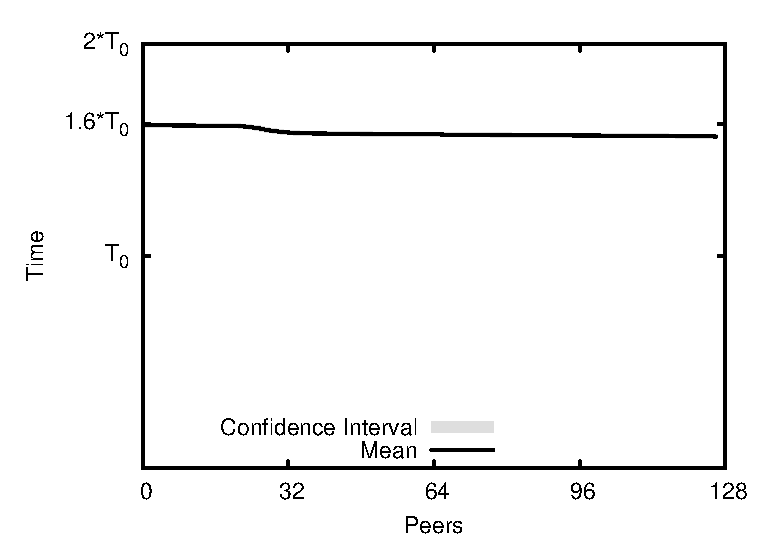
\includegraphics[width=0.5\textwidth]{plots/scenario_4_peer_count_128/plots/GeneratedMeanSortedChunkCompletion.csv}
	 	}		

	 	\subfigure[Super Seeder Upload Bandwidth\label{fig:s5:ssupload}]{
	 		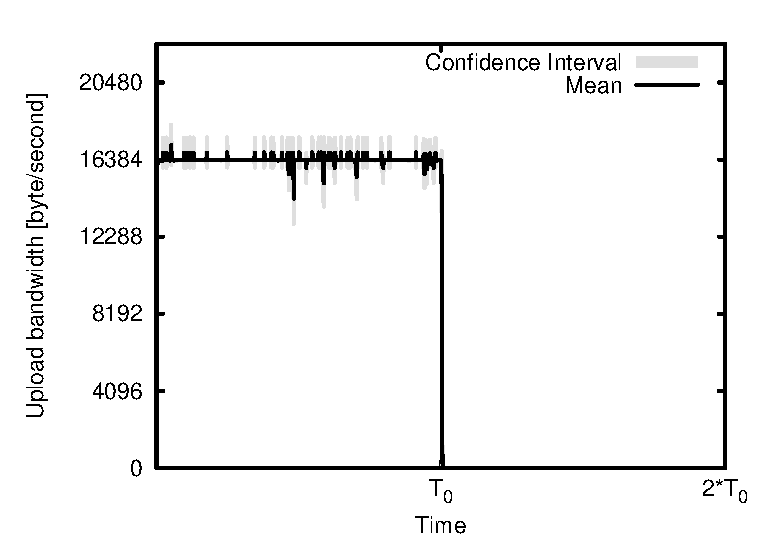
\includegraphics[width=0.5\textwidth]{plots/scenario_4_peer_count_128/plots/GeneratedMeanCurrentSuperSeederUploadBandwidth.csv}
	 	}~ % No whitespace here!
	 	\subfigure[Seeder Upload Bandwidth\label{fig:s5:upload}]{
	 		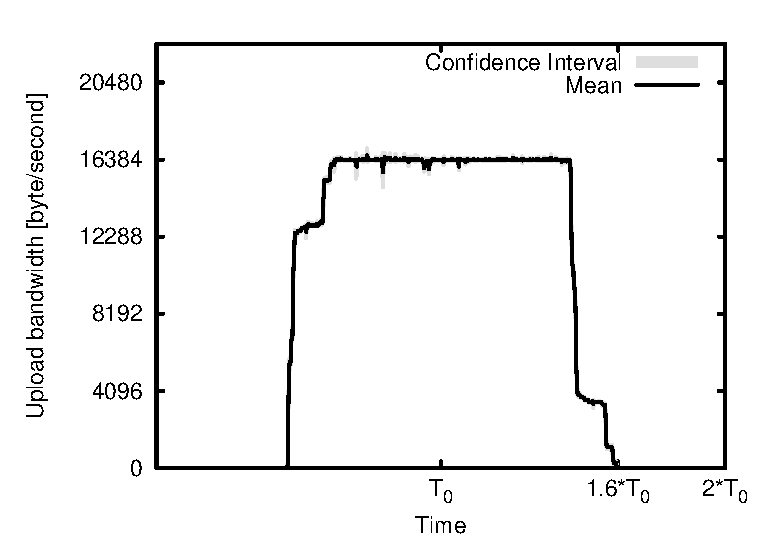
\includegraphics[width=0.5\textwidth]{plots/scenario_4_peer_count_128/plots/GeneratedMeanCurrentUploadBandwidth.csv}
	 	}

	 	\subfigure[Leecher Download Bandwidth\label{fig:s5:download}]{
	 		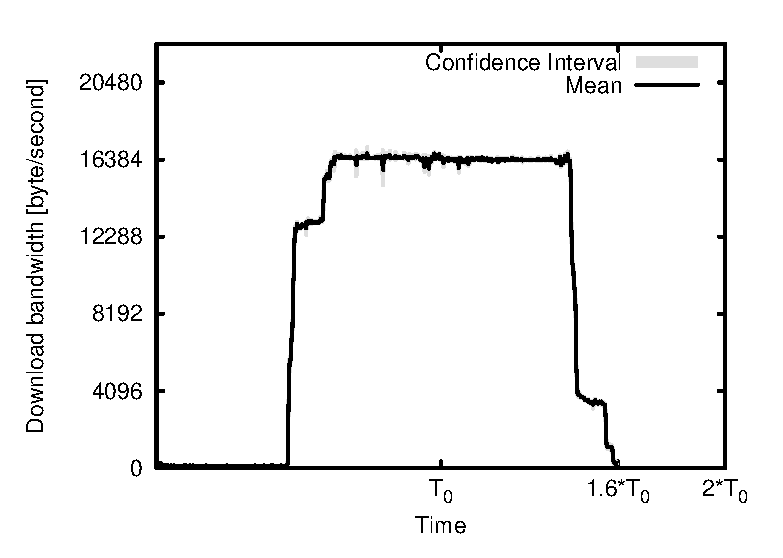
\includegraphics[width=0.5\textwidth]{plots/scenario_4_peer_count_128/plots/GeneratedMeanCurrentDownloadBandwidth.csv}
	 	}
		\caption{Scenario 5 - 128 Peers}
		\label{fig:s5}
	\end{center}
\end{figure}
\vfill

\pagebreak
\begin{figure}[!ht]
	\begin{center}	
		\subfigure[Completion Process\label{fig:s6:completion}]{
	 		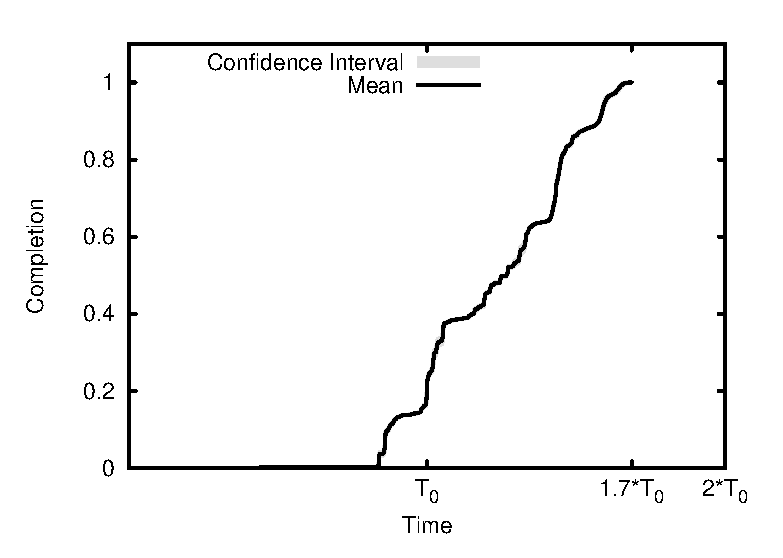
\includegraphics[width=0.5\textwidth]{plots/scenario_11_peer_count_192_v2/plots/GeneratedMeanChunkCompletion.csv}
	 	}~ % No whitespace here!
	 	\subfigure[Sorted Completion\label{fig:s6:scompletion}]{
	 		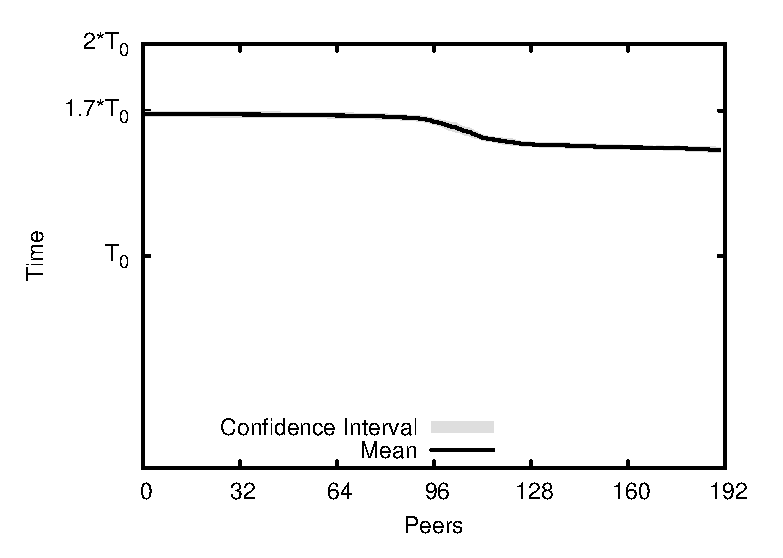
\includegraphics[width=0.5\textwidth]{plots/scenario_11_peer_count_192_v2/plots/GeneratedMeanSortedChunkCompletion.csv}
	 	}		

	 	\subfigure[Super Seeder Upload Bandwidth\label{fig:s6:ssupload}]{
	 		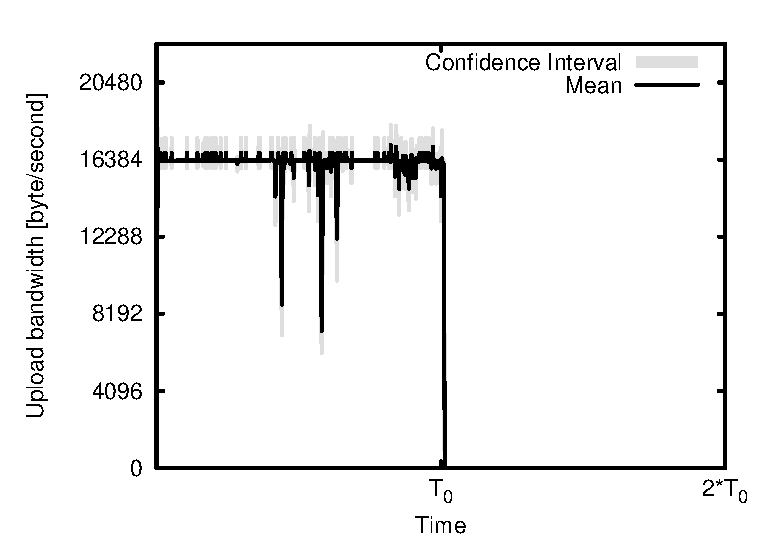
\includegraphics[width=0.5\textwidth]{plots/scenario_11_peer_count_192_v2/plots/GeneratedMeanCurrentSuperSeederUploadBandwidth.csv}
	 	}~ % No whitespace here!
	 	\subfigure[Seeder Upload Bandwidth\label{fig:s6:upload}]{
	 		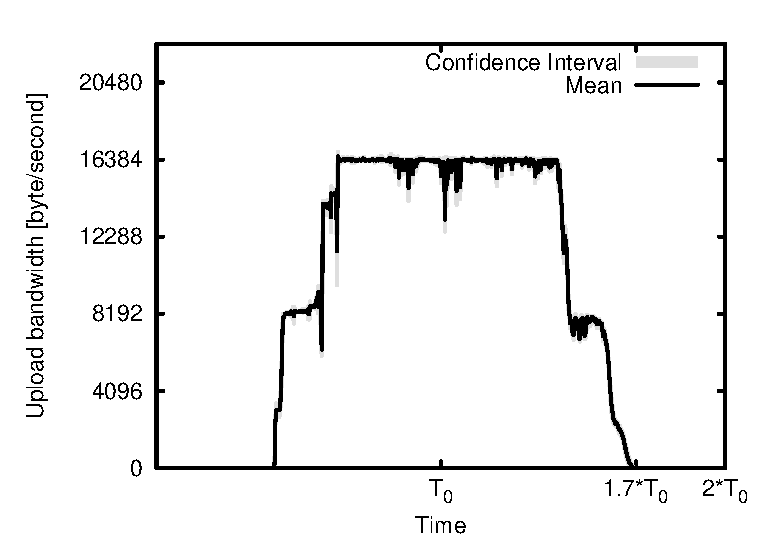
\includegraphics[width=0.5\textwidth]{plots/scenario_11_peer_count_192_v2/plots/GeneratedMeanCurrentUploadBandwidth.csv}
	 	}

	 	\subfigure[Leecher Download Bandwidth\label{fig:s6:download}]{
	 		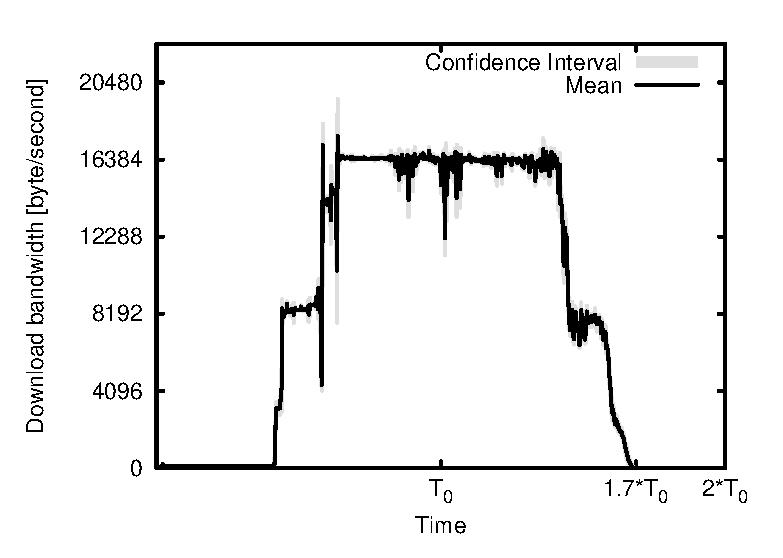
\includegraphics[width=0.5\textwidth]{plots/scenario_11_peer_count_192_v2/plots/GeneratedMeanCurrentDownloadBandwidth.csv}
	 	}
		\caption{Scenario 6 - 192 Peers}
		\label{fig:s6}
	\end{center}
\end{figure}
\vfill

\pagebreak
\section{Scenario 4, 5 and 6: Peer Count}
\label{evaluation:456}

Compared to the default scenario, scenario 4, 5 and 6 have a peer count of 32, 128 and 192 respectively. These scenarios are used to observe the large-scale behavior, whose results are shown in figure \ref{fig:s4}, \ref{fig:s5} and \ref{fig:s6}. The results from scenario 4 and the default scenario are almost identical, actually scenario 4 behaves even more as predicted. In contrast, scenario 5 and 6 show a minor decrease in performance. While the default scenario and scenario 4 both take about $1.5\:*\:T_0$ seconds, scenario 5 and 6 take $1.6\:*\:T_0$ and $1.7\:*\:T_0$ seconds respectively. While all of these scenarios do not exceed $2\:*\:T_0$ seconds, the performance obviously drops when using more peers.

The complexity of a mesh topology is ${\mathcal O(n^2)}$, which is one reason for the performance drop. If the peer count is doubled, the chunk count is doubled as well, so the number of announce messages actually quadruples. Theoretically, the Chunked-Swarm model works for any number of clients, but in practice the overhead introduced by the growing number of chunks and announce messages is just too high at some point. In reality, every announce message would also increase the latency caused by the \emph{round trip time}. 

Another reason might be unfair chunk distribution, because if a peer downloads its chunk too fast, it might download a second chunk, which should have been distributed by an other peer and thus distributes two chunks instead of one. This effect seems to happen more often under high pressure, as shown in figure \ref{fig:s5:upload} and \ref{fig:s6:upload}. Some peers start distributing their own chunks before $0.5\:*\:T_0$, while others seem to upload chunks even after $1.5\:*\:T_0$. A solution to this problem is discussed in Chapter \ref{conclusion}.

It should be noted, that the limit is not exactly 192 peers. When simulating 192 peers, the server actually runs $192\:*\:191=36.672$ connections at once, which has a great impact on CPU and main memory usage. Programmatically, there are also major reasons for the huge overhead. Since the implementation is written in Java, there is no way to allocate class instances on the stack. This is discussed in Chapter \ref{conclusion} in more detail. Also, in reality, the overhead is distributed evenly among all peers. So a single peer should be able to handle way more than 192 peers. Unfortunately, there are no results taken from real peers yet, so the last statement is just an assumption, which has yet to be proven.

\vfill



\pagebreak
\begin{figure}[!ht]
	\begin{center}	
		\subfigure[Completion Process\label{fig:s7:completion}]{
	 		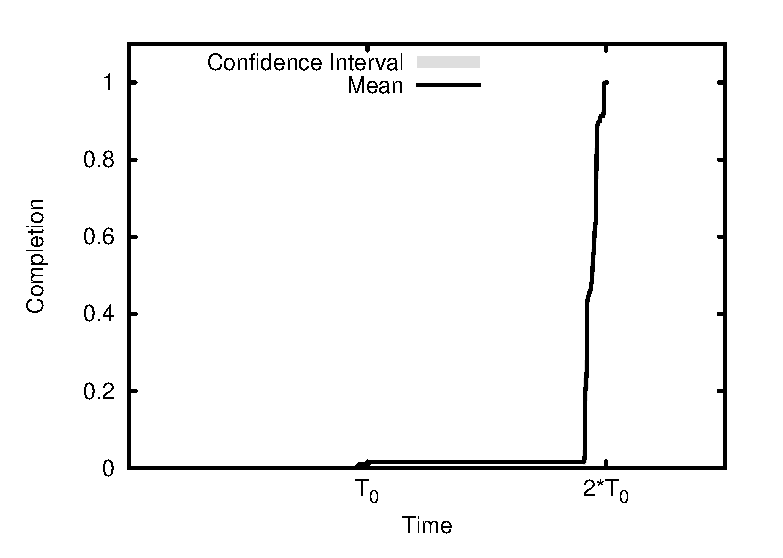
\includegraphics[width=0.5\textwidth]{plots/scenario_7_chunk_count_fac_1/plots/GeneratedMeanChunkCompletion.csv}
	 	}~ % No whitespace here!
	 	\subfigure[Sorted Completion\label{fig:s7:scompletion}]{
	 		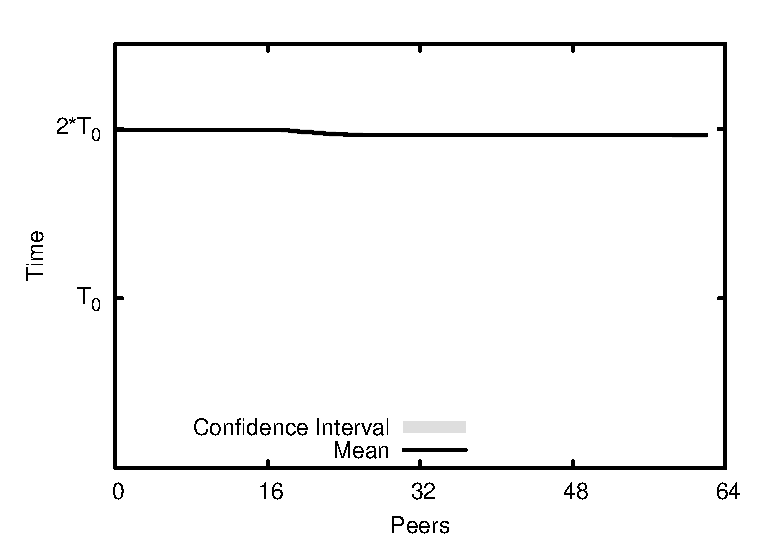
\includegraphics[width=0.5\textwidth]{plots/scenario_7_chunk_count_fac_1/plots/GeneratedMeanSortedChunkCompletion.csv}
	 	}		

	 	\subfigure[Super Seeder Upload Bandwidth\label{fig:s7:ssupload}]{
	 		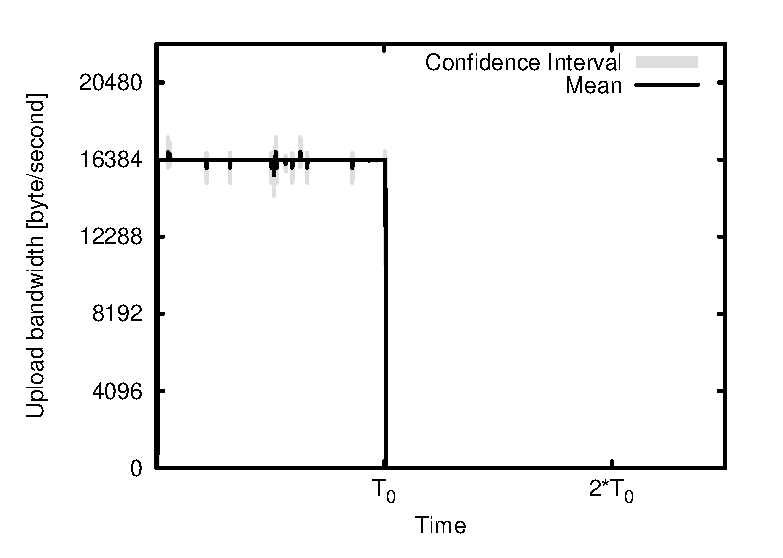
\includegraphics[width=0.5\textwidth]{plots/scenario_7_chunk_count_fac_1/plots/GeneratedMeanCurrentSuperSeederUploadBandwidth.csv}
	 	}~ % No whitespace here!
	 	\subfigure[Seeder Upload Bandwidth\label{fig:s7:upload}]{
	 		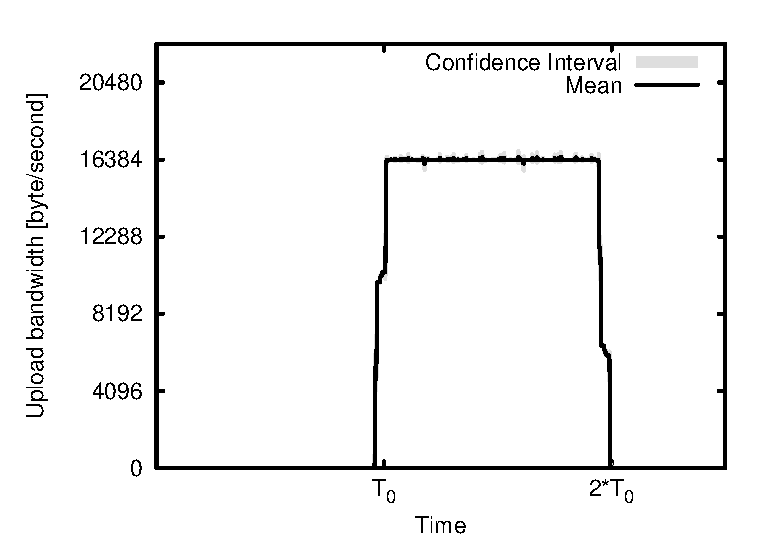
\includegraphics[width=0.5\textwidth]{plots/scenario_7_chunk_count_fac_1/plots/GeneratedMeanCurrentUploadBandwidth.csv}
	 	}

	 	\subfigure[Leecher Download Bandwidth\label{fig:s7:download}]{
	 		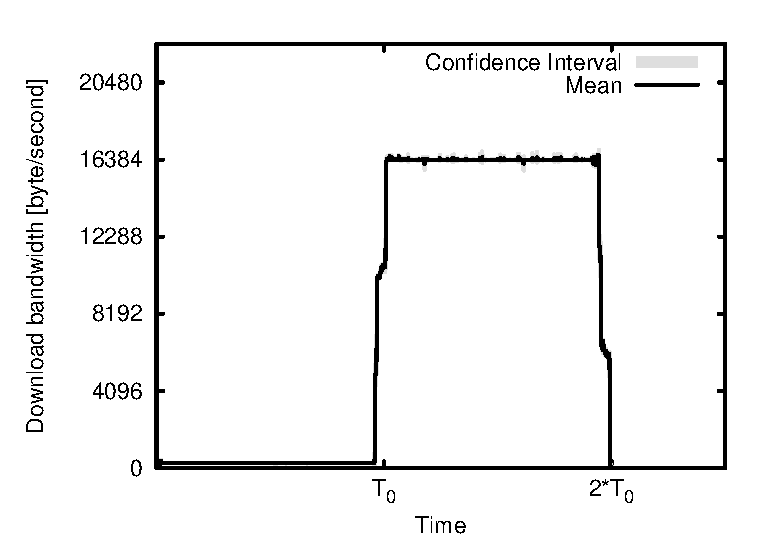
\includegraphics[width=0.5\textwidth]{plots/scenario_7_chunk_count_fac_1/plots/GeneratedMeanCurrentDownloadBandwidth.csv}
	 	}
		\caption{Scenario 7 - Chunk Count Factor 1}
		\label{fig:s7}
	\end{center}
\end{figure}
\vfill

\pagebreak
\begin{figure}[!ht]
	\begin{center}	
		\subfigure[Completion Process\label{fig:s8:completion}]{
	 		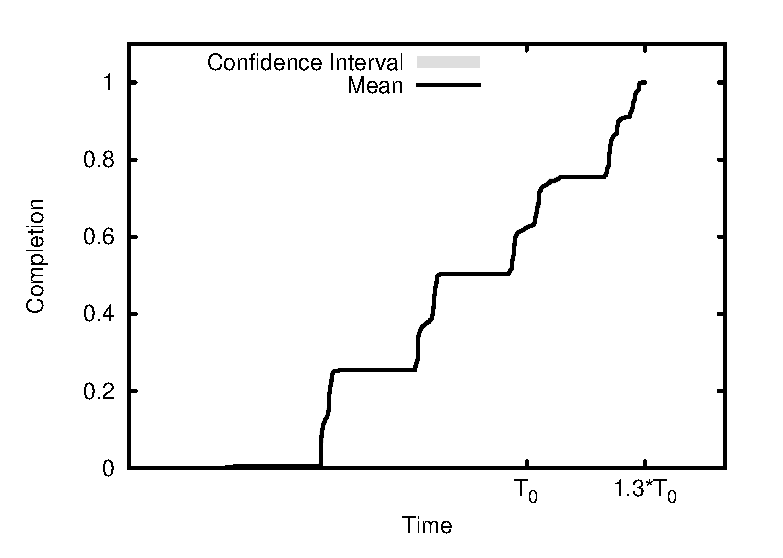
\includegraphics[width=0.5\textwidth]{plots/scenario_15_chunk_count_fac_4/plots/GeneratedMeanChunkCompletion.csv}
	 	}~ % No whitespace here!
	 	\subfigure[Sorted Completion\label{fig:s8:scompletion}]{
	 		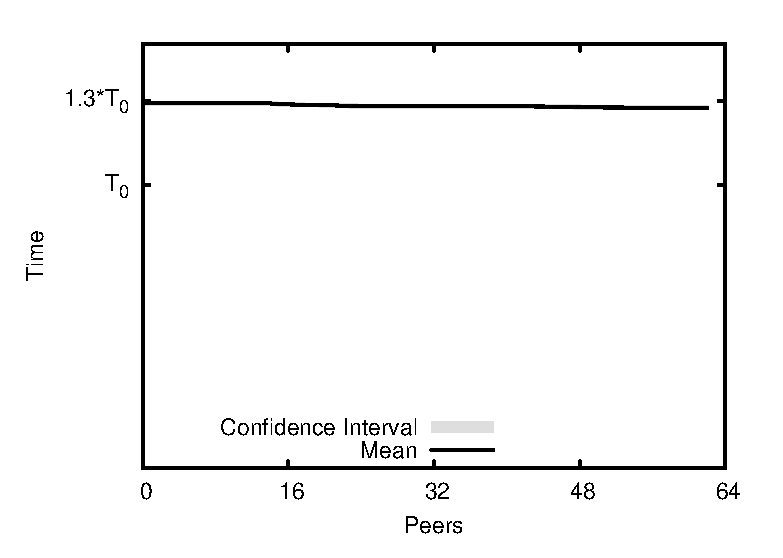
\includegraphics[width=0.5\textwidth]{plots/scenario_15_chunk_count_fac_4/plots/GeneratedMeanSortedChunkCompletion.csv}
	 	}		

	 	\subfigure[Super Seeder Upload Bandwidth\label{fig:s8:ssupload}]{
	 		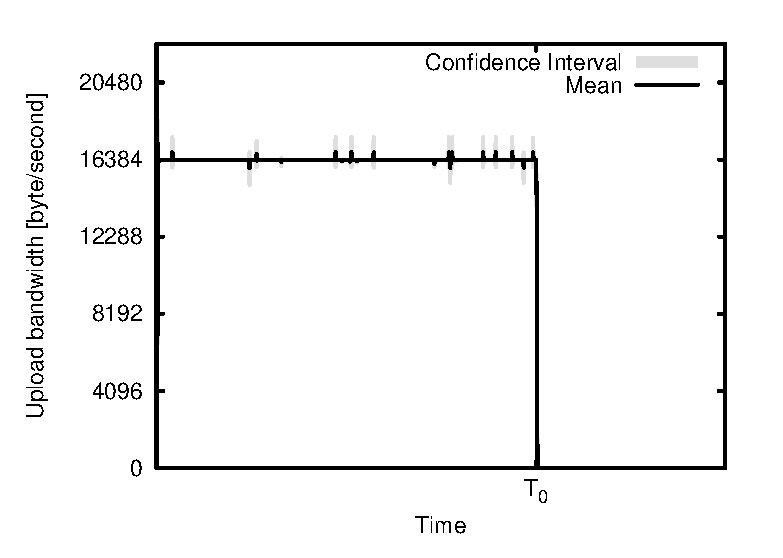
\includegraphics[width=0.5\textwidth]{plots/scenario_15_chunk_count_fac_4/plots/GeneratedMeanCurrentSuperSeederUploadBandwidth.csv}
	 	}~ % No whitespace here!
	 	\subfigure[Seeder Upload Bandwidth\label{fig:s8:upload}]{
	 		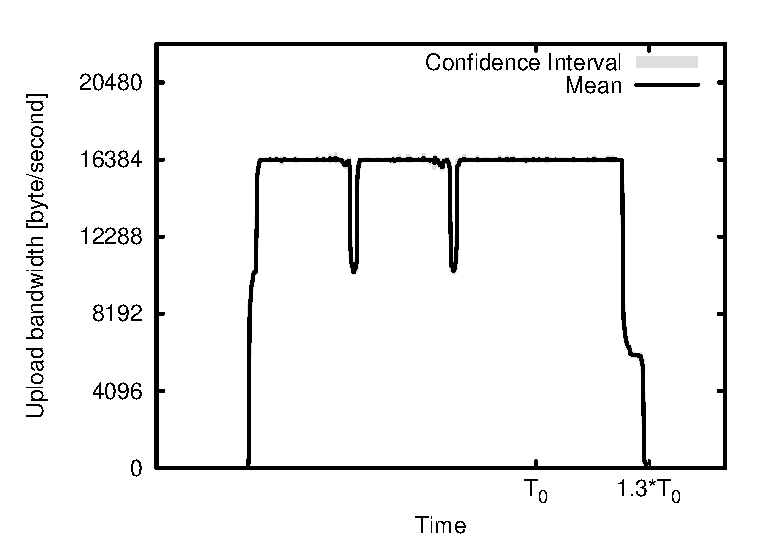
\includegraphics[width=0.5\textwidth]{plots/scenario_15_chunk_count_fac_4/plots/GeneratedMeanCurrentUploadBandwidth.csv}
	 	}

	 	\subfigure[Leecher Download Bandwidth\label{fig:s8:download}]{
	 		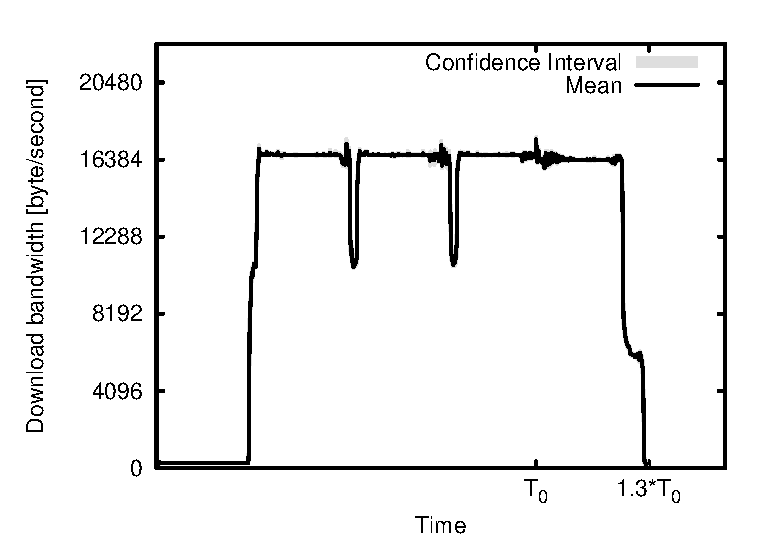
\includegraphics[width=0.5\textwidth]{plots/scenario_15_chunk_count_fac_4/plots/GeneratedMeanCurrentDownloadBandwidth.csv}
	 	}
		\caption{Scenario 8 - Chunk Count Factor 4}
		\label{fig:s8}
	\end{center}
\end{figure}
\vfill

\pagebreak
\begin{figure}[!ht]
	\begin{center}	
		\subfigure[Completion Process\label{fig:s9:completion}]{
	 		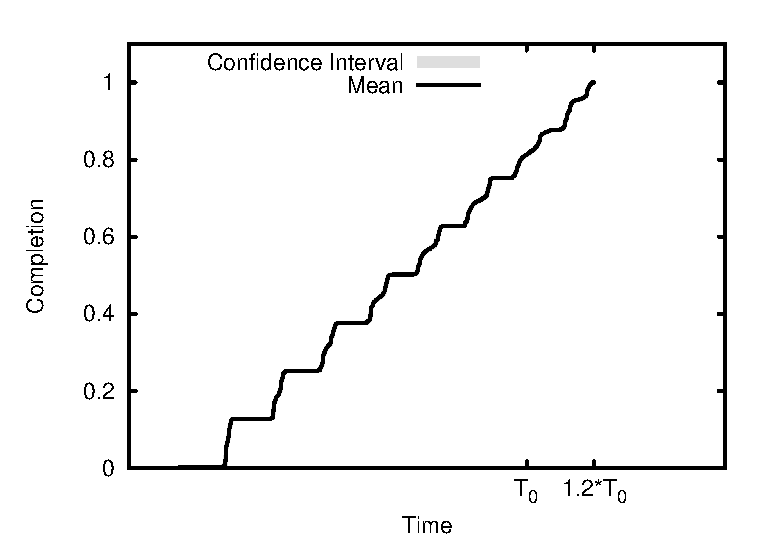
\includegraphics[width=0.5\textwidth]{plots/scenario_16_chunk_count_fac_8/plots/GeneratedMeanChunkCompletion.csv}
	 	}~ % No whitespace here!
	 	\subfigure[Sorted Completion\label{fig:s9:scompletion}]{
	 		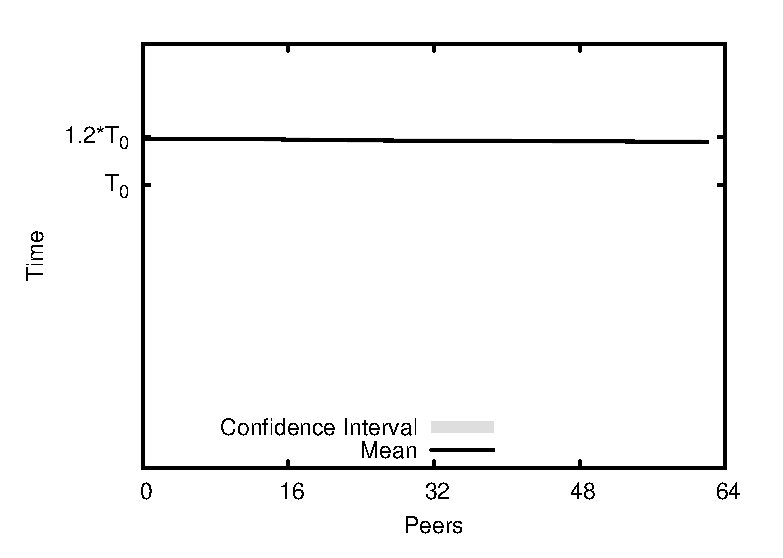
\includegraphics[width=0.5\textwidth]{plots/scenario_16_chunk_count_fac_8/plots/GeneratedMeanSortedChunkCompletion.csv}
	 	}		

	 	\subfigure[Super Seeder Upload Bandwidth\label{fig:s9:ssupload}]{
	 		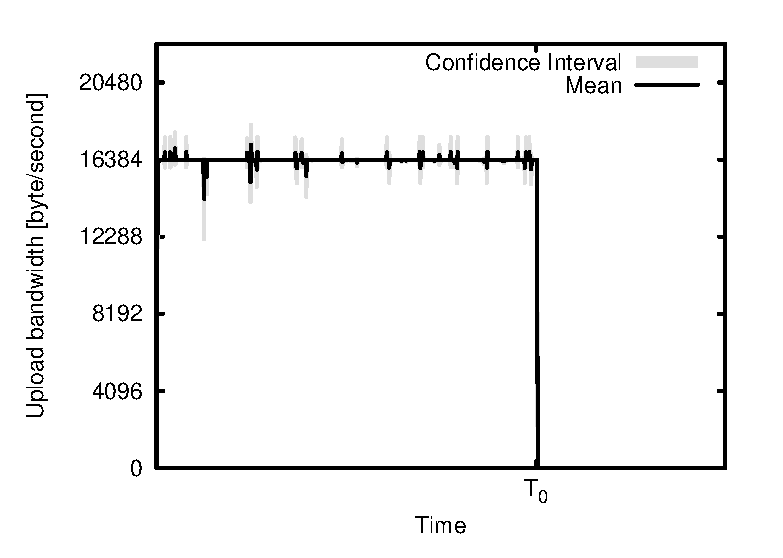
\includegraphics[width=0.5\textwidth]{plots/scenario_16_chunk_count_fac_8/plots/GeneratedMeanCurrentSuperSeederUploadBandwidth.csv}
	 	}~ % No whitespace here!
	 	\subfigure[Seeder Upload Bandwidth\label{fig:s9:upload}]{
	 		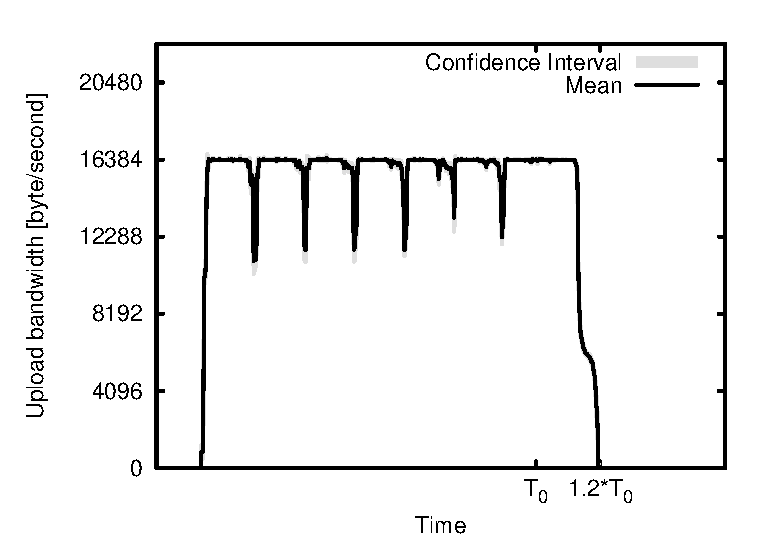
\includegraphics[width=0.5\textwidth]{plots/scenario_16_chunk_count_fac_8/plots/GeneratedMeanCurrentUploadBandwidth.csv}
	 	}

	 	\subfigure[Leecher Download Bandwidth\label{fig:s9:download}]{
	 		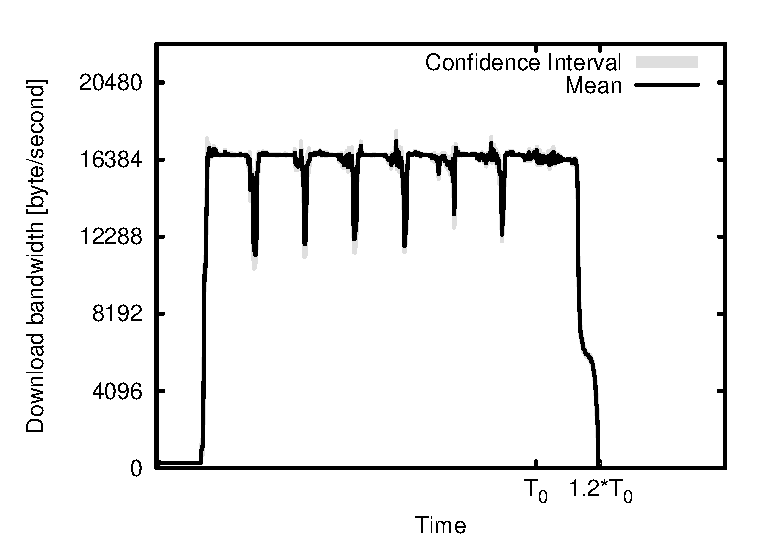
\includegraphics[width=0.5\textwidth]{plots/scenario_16_chunk_count_fac_8/plots/GeneratedMeanCurrentDownloadBandwidth.csv}
	 	}
		\caption{Scenario 9 - Chunk Count Factor 8}
		\label{fig:s9}
	\end{center}
\end{figure}
\vfill


\pagebreak
\begin{figure}[!ht]
	\begin{center}	
		\subfigure[Completion Process\label{fig:s10:completion}]{
	 		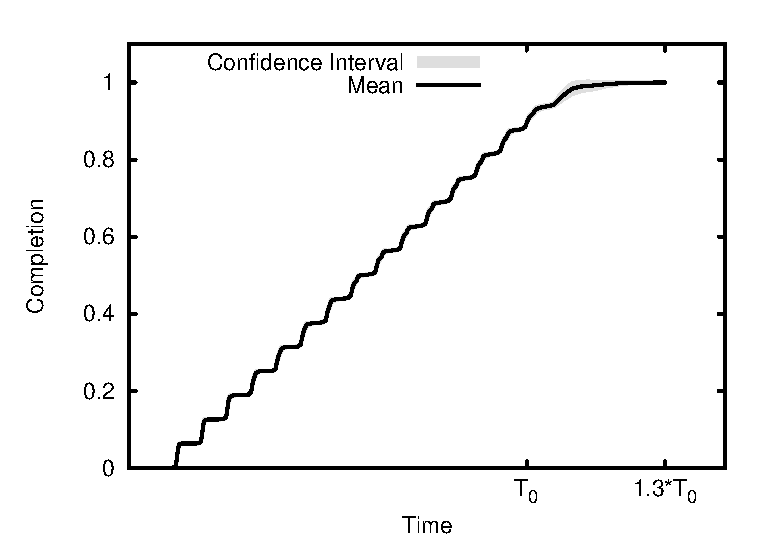
\includegraphics[width=0.5\textwidth]{plots/scenario_17_chunk_count_fac_16/plots/GeneratedMeanChunkCompletion.csv}
	 	}~ % No whitespace here!
	 	\subfigure[Sorted Completion\label{fig:s10:scompletion}]{
	 		\includegraphics[width=0.5\textwidth]{plots/scenario_17_chunk_count_fac_16/plots/GeneratedMeanSortedChunkCompletion.csv}
	 	}		

	 	\subfigure[Super Seeder Upload Bandwidth\label{fig:s10:ssupload}]{
	 		\includegraphics[width=0.5\textwidth]{plots/scenario_17_chunk_count_fac_16/plots/GeneratedMeanCurrentSuperSeederUploadBandwidth.csv}
	 	}~ % No whitespace here!
	 	\subfigure[Seeder Upload Bandwidth\label{fig:s10:upload}]{
	 		\includegraphics[width=0.5\textwidth]{plots/scenario_17_chunk_count_fac_16/plots/GeneratedMeanCurrentUploadBandwidth.csv}
	 	}

	 	\subfigure[Leecher Download Bandwidth\label{fig:s10:download}]{
	 		\includegraphics[width=0.5\textwidth]{plots/scenario_17_chunk_count_fac_16/plots/GeneratedMeanCurrentDownloadBandwidth.csv}
	 	}
		\caption{Scenario 10 - Chunk Count Factor 16}
		\label{fig:s10}
	\end{center}
\end{figure}
\vfill

\pagebreak
\section{Scenario 7, 8, 9 and 10: Chunk Count Factor}
\label{evaluation:78910}

In scenario 7, 8, 9 and 10 the chunk count factor is adjusted to 1, 4, 8 and 16 respectively. The chunk count factor is multiplied with the number of peers, but without the super seeder, to calculate the actual chunk count. The default scenario uses a chunk count factor of 2 and a peer count of 63, without the super seeder. Since these four scenarios only change the chunk count factor, the used chunk counts are $1\:*\:63$, $4\:*\:63=252$, $8\:*\:63=504$ and $16\:*\:63=1008$ for scenario 7, 8, 9 and 10 respectively.   

As expected, scenario 7 completes in $2\:*\:T_0$, see figure \ref{fig:s7}. In the first $T_0$ seconds the super seeder uploads a distinct chunk to each peer, whereby the complete data set is available in the network. Since the super seeder is not allowed to upload the same chunk twice, the peer have to distribute all chunks evenly among themselves, which also takes roughly $T_0$ seconds. These results correspond with the formula presented in \ref{theory:model:chunkedswarm}, because $c\:=63$, $n\:=\:63$ and $T(63, 63) = (1\:+\:\frac{63-1}{63})\:T_0 = 1,98\:T_0$.

Scenario 8, whose results are shown in figure \ref{fig:s8}, completed in $1.3\:*\:T_0$, which is almost the expected duration, since $c\:=252$, $n\:=\:63$ and $T(63, 252) = (1\:+\:\frac{63-1}{252})\:T_0 = 1,25\:T_0$. But it is important to note, that at with chunk count factor of 4, the completion graph already starts to leave the expected path, which should have been a step function with four steps, starting at $0.25\:*\:T_0$. As with Scenario 5 and 6, this effect gets worse under high pressure. The unfair chunk distribution also gets worse, if more chunks are involved. So while the overall distribution time shrinks, the system as a whole gets more fragile.

Scenario 9 and 10 are even more fragile, as shown in figure \ref{fig:s9} and \ref{fig:s10}. The expected durations are $(1\:+\:\frac{63-1}{504})\:T_0 = 1,12\:T_0$ and $(1\:+\:\frac{63-1}{1008})\:T_0 = 1,06\:T_0$ respectively. Even worse, scenario 10 takes longer than scenario 9 on average. While scenario 9 is barely acceptable, scenario 10 has a new influence, that should be noted. As explained before, the results are calculated from ten runs. At this point, all ten runs of all scenarios completed mostly identical, which is represented by the low confidence interval. This changes dramatically in scenario 10. Some runs completed at $1.5\:*\:T_0$, while the majority completed at $1.08\:*\:T_0$. This means, that some runs behaved much worse than the others. The raw results let assume, that unfair chunk distribution is now the main reason for that. Figure \ref{fig:s10:scompletion}, \ref{fig:s10:upload} and \ref{fig:s10:download} contain these high confidence interval areas. 

In theory, if the chunk count is doubled, the completion time after $T_0$ will cut in half. Scenario 1, 7, 8 and 9 confirm this assumption. But it seems, that unfair chunk distribution can make the system really fragile. Since this problem occurs under high pressure in every scenario, a more stable implementation has to be found.

\vfill


\pagebreak
\begin{figure}[!ht]
	\begin{center}	
		\subfigure[Completion Process\label{fig:s11:completion}]{
	 		\includegraphics[width=0.5\textwidth]{plots/scenario_9_parts_10/plots/GeneratedMeanChunkCompletion.csv}
	 	}~ % No whitespace here!
	 	\subfigure[Sorted Completion\label{fig:s11:scompletion}]{
	 		\includegraphics[width=0.5\textwidth]{plots/scenario_9_parts_10/plots/GeneratedMeanSortedChunkCompletion.csv}
	 	}		

	 	\subfigure[Super Seeder Upload Bandwidth\label{fig:s11:ssupload}]{
	 		\includegraphics[width=0.5\textwidth]{plots/scenario_9_parts_10/plots/GeneratedMeanCurrentSuperSeederUploadBandwidth.csv}
	 	}~ % No whitespace here!
	 	\subfigure[Seeder Upload Bandwidth\label{fig:s11:upload}]{
	 		\includegraphics[width=0.5\textwidth]{plots/scenario_9_parts_10/plots/GeneratedMeanCurrentUploadBandwidth.csv}
	 	}

	 	\subfigure[Leecher Download Bandwidth\label{fig:s11:download}]{
	 		\includegraphics[width=0.5\textwidth]{plots/scenario_9_parts_10/plots/GeneratedMeanCurrentDownloadBandwidth.csv}
	 	}
		\caption{Scenario 11 - Streaming 10 Data Sets}
		\label{fig:s11}
	\end{center}
\end{figure}
\vfill


\pagebreak
\begin{figure}[!ht]
	\begin{center}	
		\subfigure[Completion Process\label{fig:s12:completion}]{
	 		\includegraphics[width=0.5\textwidth]{plots/scenario_6_parts_20/plots/GeneratedMeanChunkCompletion.csv}
	 	}~ % No whitespace here!
	 	\subfigure[Sorted Completion\label{fig:s12:scompletion}]{
	 		\includegraphics[width=0.5\textwidth]{plots/scenario_6_parts_20/plots/GeneratedMeanSortedChunkCompletion.csv}
	 	}		

	 	\subfigure[Super Seeder Upload Bandwidth\label{fig:s12:ssupload}]{
	 		\includegraphics[width=0.5\textwidth]{plots/scenario_6_parts_20/plots/GeneratedMeanCurrentSuperSeederUploadBandwidth.csv}
	 	}~ % No whitespace here!
	 	\subfigure[Seeder Upload Bandwidth\label{fig:s12:upload}]{
	 		\includegraphics[width=0.5\textwidth]{plots/scenario_6_parts_20/plots/GeneratedMeanCurrentUploadBandwidth.csv}
	 	}

	 	\subfigure[Leecher Download Bandwidth\label{fig:s12:download}]{
	 		\includegraphics[width=0.5\textwidth]{plots/scenario_6_parts_20/plots/GeneratedMeanCurrentDownloadBandwidth.csv}
	 	}
		\caption{Scenario 12 - Streaming 20 Data Sets}
		\label{fig:s12}
	\end{center}
\end{figure}
\vfill

\pagebreak
\section{Scenario 11 and 12: Streaming Multiple Data Sets}
\label{evaluation:1112}

So far, all other scenarios used and transferred only one data set. The last scenarios 11 and 12 implement the streaming of 10 and 20 data sets respectively, see Section \ref{theory:model:chunkedswarm} and \ref{module:streaming}. The data sets are much smaller now and thus complete in less time.

In case of scenario 11, each data set takes $\frac{1}{10}\:*\:T_0$ seconds to get from one peer to another. So transferring all data sets take $T_0$ seconds. Therefore, the peers download ten data sets from the super seeder and distribute them one after the other. This is useful to implement sequential streaming, where a huge data source is splitted into multiple data sets, which are downloaded and distributed sequentially so that each peer do not have random chunks but a growing amount of coherent chunks instead. Video streaming is only one domain, which relies on this behavior.

Figure \ref{fig:s11} shows the results from scenario 11. An interesting observation is, that all peers finish within $1.2\:*\:T_0$ seconds, but each data set has a chunk count factor of 2. The reason is, that the download and the distribution phases of each data set interleave. So the super seeder starts uploading the next data set while the peers are still distributing the last data set, which is shown in figure \ref{fig:s11:ssupload}, \ref{fig:s11:upload} and \ref{fig:s11:download}. The high confidence intervals are caused by the large amount of chunks. When simulating ten runs, it is very unlikely, that all results are equal. But the confidence intervals show, that it is still very likely, that a further run will be very similar. The completion graphs \ref{fig:s11:completion} and \ref{fig:s11:scompletion} also show the good distribution behavior. All peers download and distribute the data sets equally. Figure \ref{fig:s12} contains the results from scenario 12, which has 20 data sets instead of 10. The results are very similar to those from scenario 11, so there is not much to say about it.

While the results of both scenarios look promising, it should be noted, that both scenarios run 20 times instead of 10. Then only the best 10 runs were chosen and merged. The reason is, that some runs took about $4\:*\:T_0$ to $6\:*\:T_0$ seconds to finish, while others took roughly $1.2\:*\:T_0$ seconds. In case of the slow scenarios, the results show, that most of the peers were not uploading anymore after $1.5\:*\:T_0$ seconds, which is the reason why these runs took so long. So the graphs of both scenarios show, that it is possible to get the expected performance, but the system is also very fragile and can get out of step. Again, the main reason for this effect is unfair chunk distribution. In the next Chapter \ref{conclusion} a push based approach is proposed, which should solve this particular problem in the future.

\cleardoublepage
%!TEX root = bachelor.tex

\chapter{Conclusion}
\label{conclusion}

As shown in Chapter \ref{evaluation}, the implementation of the Chunked-Swarm model using the super seeder extension, discussed in \ref{theory:model:chunkedswarm}, is able to distribute data sets among a variable number of peers within $2\:*\:T_0$ seconds, where $T_0$ is the time for transferring a data set from one peer to another. In some scenarios, this model is even able to undercut the $2\:*\:T_0$ limit by far. Since all benchmarks ran in real-time, a high CPU usage caused by scenarios with many peers or a high chunk count can affect the significance of the results of these scenarios, which relates to exponentially growing overhead caused by the mesh topology. To minimize the impact of a high CPU usage, a simulation time should be implemented, to simulate even hundreds and thousands of peers.

If the CPU is fully utilized, thread scheduling is not fair anymore, so some peers can get more time to operate than others. This could lead to unfair chunk distribution, where one peer distributes more chunks as it should, while another peer distribute nothing at all. Thus, the solution works fine in general, but might drop performance under high CPU load. The main reason for this effect is the pull-based approach. Every peer explicitly request chunks from other peers. At first, only the super seeder can offer chunks. The peers receive announcements and start downloading chunks from the super seeder. These chunks are distinct from each other, because the super seeder rejects download requests of chunks, which have already been uploaded to other peers. Then, every peer announces and uploads its own chunk to the other peers. If a peer A completes its chunk download from the super seeder too early, it might happen, that another peer B requests this chunk from peer A, which will be transferred really fast, since there is no other peer requesting this chunk yet. Then, the other peers try to download the chunk and notice, that there are two peers offering this chunk. If peer A just finished another chunk, the remaining peers would request the chunk from peer B, because a chunk is always requested from the peer, which offers least. But at some point, peer B will have its own distinct chunk from the super seeder as well. This chunk must be distributed by peer B, because no one else has this chunk. This means, peer B is now responsible for two chunks, while peer A is waiting for requests. A large number of peers or a high chunk count factor can increase the possibility for this situation.

Unfortunately, this is a fundamental problem of the pull-based approach, because the peers do not know which chunks other peers request. While this approach is good to prevent chunk duplication, see \ref{module:algorithm:chunkedswarm}, it ignores some information the system already knows. If a peer A successfully downloads a chunk from the super seeder, this chunk is not present in the Peer-to-Peer network yet. So this chunk must be distributed through peer A. Also, peer A basically knows, that all other peers want this chunk as well, so waiting for explicit requests seems counterintuitive. A push-based approach would solve these issues. A peer pushes chunks from the super seeder to every other peer in the network. But a peer is not allowed to push a chunk, that was not received from the super seeder earlier. This way, the load is distributed evenly across all peers. Also, there is no need for chunk announcements anymore, which are described in Section \ref{module:core:net:annoucements}. Therefore, the system scales better, while latency is reduced significantly.

Another problem is the Java programming language. As explained in Section \ref{evaluation:456}, Java does not support stack allocation of class instances. Since the pull-based approach creates many small data structures, the heap memory of the application grows rapidly and thus causes garbage collection to run more often. The impact has been observed using the \emph{JVisualVM}\footnote{http://docs.oracle.com/javase/6/docs/technotes/tools/share/jvisualvm.html} tool provided by \emph{Oracle}. A future implementation is strongly encouraged to implement some sort of manual object pooling or to use a runtime, which supports stack allocations in the first place.

%%%%%%%%%%%%%%%%%%%%%%%%%%%%%%%%%%%%%%%%%%%%%%
%%    End of the main document              %%
%%%%%%%%%%%%%%%%%%%%%%%%%%%%%%%%%%%%%%%%%%%%%%

\backmatter

\bibliographystyle{alphadin} %% german output

\bibliography{bibtex-references}

% \printindex

%!TEX root = bachelor.tex

\chapter*{Ehrenwörtliche Erklärung}

Hiermit versichere ich, die vorliegende Bachelorarbeit selbstständig 
verfasst und keine anderen als die angegebenen Quellen und Hilfsmittel
benutzt zu haben.
Alle Stellen, die aus den Quellen entnommen
wurden, sind als solche kenntlich gemacht worden. Diese Arbeit hat in
gleicher oder ähnlicher Form noch keiner Prüfungsbehörde vorgelegen.

\vspace{3cm}

\noindent Düsseldorf, 6.\thesissubmissionmonth{} \thesissubmissionyear{} \hfill \thesisauthor{}


\cleardoublepage

%!TEX root = bachelor.tex

\chapter*{}
\thispagestyle{empty}

\begin{center}
  \vspace{-3cm}
  \fbox{\parbox[c][12cm][c]{12cm}{\centering Please add here\\[1cm] the DVD holding sheet}}
\end{center}

\vfill

\textbf{This DVD contains:}
\begin{itemize}
 \item A \emph{pdf} Version of this bachelor thesis
 \item All \LaTeX\:and graphic files that have been used, as well as the corresponding scripts
 \item The source code of the software that was created during the bachelor thesis 
 \item The measurement data that was created during the evaluation
\end{itemize}


\end{document}

